\documentclass[ms,twoside,print]{nuthesis}
% Note: Leaving out print or twoside will result in oneside printing.

% ===================== Packages =====================
\usepackage{amsmath}
\usepackage{amsfonts}
\usepackage[sc,osf]{mathpazo}
\usepackage{microtype}
\usepackage{booktabs}
\usepackage{paralist}
\usepackage{graphicx}
\usepackage{xcolor}
\usepackage{float} % for [H] placement if desired
\usepackage{tikz} % Diagrams
\usetikzlibrary{arrows.meta,positioning,shapes.geometric,fit,matrix}
\usepackage{siunitx} % Optional but useful
\sisetup{detect-all}
\PassOptionsToPackage{hyphens}{url} % Make long URLs break better in refs (must come before hyperref)
\usepackage{hyperref}
\usepackage[T1]{fontenc}
\usepackage[utf8]{inputenc}
\usepackage[nameinlink,capitalize,noabbrev]{cleveref}
\usepackage{bookmark} % better PDF outlines
\usepackage{csquotes} % for \enquote
\usepackage{tabularx} % better tables that auto-wrap
\urlstyle{same}
\usepackage{listings}
\usepackage{lstautogobble} % trims common indent
\usepackage{array}
\usepackage{tabularx}
\usepackage{makecell}
\usepackage{subcaption} % defines the subfigure environment
\usepackage{placeins}
\lstset{
  basicstyle=\ttfamily\footnotesize,
  breaklines=true,
  breakatwhitespace=false, % Allow breaks anywhere (fixes long strings like connection URLs)
  breakindent=20pt, % Indent wrapped lines for better readability in .cs files
  postbreak=\raisebox{0ex}[0ex][0ex]{\ensuremath{\color{gray}\hookrightarrow\space}}, % Subtle continuation arrow for wrapped lines
  columns=fixed, % Changed to fixed for true monospace and even frame lines (prevents uneven extensions)
  keepspaces=true,
  showstringspaces=false,
  frame=single,
  framerule=0.5pt, % Thinner frame rule to reduce visual emphasis on any minor irregularities
  rulecolor=\color{gray}, % Gray frame for subtlety
  framesep=5pt, % Inner padding to keep content from edges
  autogobble=true,
  xleftmargin=5pt, % Slightly wider left margin to prevent hugging
  xrightmargin=5pt, % Matching right margin
  tabsize=4 % Standardize tabs (fixes potential "weird" alignment in .cs code)
}

% Minimal JSON + YAML languages (pretty enough, no external deps)
\lstdefinelanguage{json}{
  string=[s]{"}{"},
  comment=[l]{//},
  morecomment=[s]{/*}{*/},
  literate=
   *{0}{{{\color{black}0}}}{1}
    {1}{{{\color{black}1}}}{1}
    {2}{{{\color{black}2}}}{1}
    {3}{{{\color{black}3}}}{1}
    {4}{{{\color{black}4}}}{1}
    {5}{{{\color{black}5}}}{1}
    {6}{{{\color{black}6}}}{1}
    {7}{{{\color{black}7}}}{1}
    {8}{{{\color{black}8}}}{1}
    {9}{{{\color{black}9}}}{1}
}

\lstdefinelanguage{yaml}{
  comment=[l]{\#},
  morestring=[b]',
  morestring=[b]"
}
% C# language definition for better syntax handling
\lstdefinelanguage{CSharp}{
  morekeywords={abstract, as, base, bool, break, byte, case, catch, char, checked, class, const, continue, decimal, default, delegate, do, double, else, enum, event, explicit, extern, false, finally, fixed, float, for, foreach, goto, if, implicit, in, int, interface, internal, is, lock, long, namespace, new, null, object, operator, out, override, params, private, protected, public, readonly, ref, return, sbyte, sealed, short, sizeof, stackalloc, static, string, struct, switch, this, throw, true, try, typeof, uint, ulong, unchecked, unsafe, ushort, using, virtual, void, volatile, while},
  sensitive=true,
  morecomment=[l]{//},
  morecomment=[s]{/*}{*/},
  morestring=[b]",
  morestring=[b]',
  literate=
   *{0}{{{\color{black}0}}}{1}
    {1}{{{\color{black}1}}}{1}
    {2}{{{\color{black}2}}}{1}
    {3}{{{\color{black}3}}}{1}
    {4}{{{\color{black}4}}}{1}
    {5}{{{\color{black}5}}}{1}
    {6}{{{\color{black}6}}}{1}
    {7}{{{\color{black}7}}}{1}
    {8}{{{\color{black}8}}}{1}
    {9}{{{\color{black}9}}}{1},
}
\lstset{
  language=CSharp,  % Set default to CSharp for .cs files
  keywordstyle=\color{blue}\bfseries,
  commentstyle=\color{green!60!black},
  stringstyle=\color{red},
  numbers=none % Remove line numbers to match original setup and avoid extra left space that could offset frames
}
\newcolumntype{L}[1]{>{\raggedright\arraybackslash}p{#1}}
\newcolumntype{Y}{>{\raggedright\arraybackslash}X}
% --- Safe placeholders + brand names ---
\newcommand{\ph}[1]{\textit{<#1>}} % use like \ph{value}, never triggers math mode
\newcommand{\Brand}[1]{\mbox{#1}} % keep vendor names from awkward hyphenation
% Colors for links
\definecolor{dark-red}{rgb}{0.6,0,0}
\definecolor{dark-green}{rgb}{0,0.6,0}
\definecolor{dark-blue}{rgb}{0,0,0.6}
\interfootnotelinepenalty=10000 % Prevent breaking footnotes across pages
% --- SAFE MaybeImage macro (replaces the old one) ---
\newcommand{\MaybeImage}[2][\linewidth]{%
\begingroup
\def\imgA{#2}%
\def\imgB{images/#2}%
\IfFileExists{\imgA}{%
\includegraphics[width=#1]{\imgA}%
  }{%
\IfFileExists{\imgB}{%
\includegraphics[width=#1]{\imgB}%
    }{%
\fbox{%
\parbox[c][0.25\textheight][c]{#1}{\centering
\small Placeholder (file missing)\\[2pt]\texttt{\detokenize{#2}}\\[2pt]
          Add this image to \texttt{images/}}
      }%
    }%
  }%
\endgroup
}
% Graphics path
\graphicspath{{images/}}

% Hyperref setup
\hypersetup{
    pdfauthor={Andrei Modiga},
    pdftitle={Final Project Report: AI-Assisted Grading System Using Large Language Models},
    pdfsubject={Education and AI},
    pdfkeywords={LaTeX, Final Report, AI, Education, Grading, GPT-4o, OCR},
    linkcolor=dark-blue,
    citecolor=dark-blue,
    urlcolor=dark-red,
    colorlinks=true,
    plainpages=false
}

% Quiet memoir footer warning by giving the footer some space
\setlength{\footskip}{18pt}

\begin{document}

% ===================== Front Matter =====================
\frontmatter

\title{Final Project Report: Developing an AI-Assisted Grading System Using Large Language Models}
\author{Andrei Modiga}
\adviser{Scot Anderson, Ph.D.}
\adviserAbstract{Scot Anderson, Ph.D.}
\major{Computer Science}
\degreemonth{August}
\degreeyear{2025}
\doctype{FINAL PROJECT REPORT}

\maketitle

\begin{abstract}
We present a grading system that accelerates evaluation of open-ended student work across scanned and digital workflows. The system crops answer regions from PDFs, assigns submissions via OCR on identity regions only, and groups answers by visual semantics using a vision LLM. Instructors review and edit groups, apply rubric items once per group, and export grades from an on-screen table. The solution integrates Ghostscript rasterization, PdfPig page orchestration, SkiaSharp region extraction, Tesseract identity OCR, and GPT-4o Vision for grouping\cite{ghostscript,pdfpig,skiasharp,tesseract,openai-gpt4o}. We detail the architecture, token-budgeted batching strategy, and persistence design, then describe testing results for grouping quality, time-on-task, and usability. The approach avoids brittle handwriting OCR while preserving instructor control, fairness, and auditability.
\end{abstract}

\setcounter{tocdepth}{2}
\tableofcontents
\listoffigures
\listoftables

% ===================== Main Matter =====================
\mainmatter

% -------------------------------------------------
\chapter{Introduction and Motivation}
\section{Problem Statement}
Grading open-ended student work (handwritten or typed) is time-consuming, repetitive, and error-prone under deadline pressure. In large classes, feedback latency diminishes learning value. Typical bottlenecks include: (i) organizing mixed-format submissions (bulk scans vs.\ individual PDFs), (ii) locating answer regions for consistent review, and (iii) repeatedly applying identical rubric deductions to similar mistakes. Handwriting OCR is brittle, often forcing manual review even for simple cases.

\section{Specific Project Goals/Requirements}
This project delivers a practical, instructor-in-the-loop grading system that:
\begin{compactitem}
  \item \textit{Bulk Scans (Filled-form):} PDFs are split by known page counts. Ghostscript rasterizes pages; PdfPig validates page counts; SkiaSharp crops defined regions to PNGs.
  \item \textit{Identity OCR (filled-form only):} Tesseract extracts name/ID from a designated identity region to auto-assign submissions; unresolved items fall back to a manual pick-list. No OCR is performed on answers; grouping uses GPT-4o Vision directly on the cropped images.
  \item \textit{Identity Matching:} (filled-form) identity text is matched to the class roster; (free-form) uploads are automatically tied to the uploader's account.
  \item \textit{Editable AI Assistance:} Vision LLM proposes semantic groups; instructors can merge/split groups, move answers, and apply rubric items per-group.
  \item \textit{Traceability:} All actions and groupings are persisted with timestamps for audit; grades are summarized in an on-screen table for review/copy.
\end{compactitem}

\section{Motivation and Benefits}
\begin{compactitem}
  \item \textbf{Faster feedback:} Instructors grade clusters of similar answers once, reducing turnaround time.
  \item \textbf{Consistency:} Per-group rubric application reduces drift across similar answers and sessions.
  \item \textbf{Lower cognitive load:} The system automates extraction, grouping suggestions, and grade totals; instructors focus on assessment.
  \item \textbf{Reduced brittleness:} Avoiding handwriting OCR on answers eliminates a major failure mode.
  \item \textbf{Privacy-aware:} Only identity crops contain PII; answer crops are devoid of names or IDs.
\end{compactitem}

\section{Contributions}
\begin{compactitem}
  \item An \textbf{OCR-minimal}, vision-first pipeline that uses OCR only for identity assignment.
  \item A \textbf{token-budgeted batching} strategy (downscale + tiling) to bound latency/cost at class scale.
  \item A \textbf{traceable data model \& APIs} with idempotent re-uploads and stable crop filenames.
  \item An \textbf{instructor-in-the-loop} UX with editable groups, explicit review status, and rubric-first grading.
\end{compactitem}

\section{Assumptions and Scope}
We target short-answer problems with recognizable visual structure (boxes/lines). Free-form essays are supported via uploaded PDFs but are not auto-scored; the system focuses on grouping to speed human grading. We assume class rosters are available and that instructors can define answer regions once per assignment.

\section{Report Organization}
\Cref{chap:bg} reviews related work and context. \Cref{chap:solution} details the system, \Cref{chap:evalplan} presents the evaluation plan, \Cref{chap:results} reports results, and the final chapter concludes with future work.

% -------------------------------------------------
\chapter{Background and Context}\label{chap:bg}
\section{AI in Education}
AI has long promised efficiency gains and personalization in education, from adaptive tutoring to analytics that help instructors intervene earlier. Reviews highlight benefits such as individualized practice, faster feedback, and administrative automation when deployed with appropriate oversight\cite{Alto2023,Chen2020,Luckin2016,Zawacki2019}. Ensuring teachers can review and revise AI-generated grades—and retain final say to confirm fairness—is essential for trust and real learning gains.

\section{Automated Grading of Short Answers and Essays}
Pre-LLM systems typically relied on feature engineering, keyword overlap, or supervised models trained on labeled answers. These reduce load but struggle with paraphrase and reasoning variance\cite{Weegar2022,Konnecke2020}. Clustering similar answers to grade in batches is a recurring theme: once clusters form, instructors can assign rubrics at the group level.

\section{LLMs and GPT-4/4o for Assessment}
Recent work investigates LLMs for grading and feedback across STEM and writing tasks. Studies report promising alignment with human graders for mathematical reasoning and physics solutions when prompts focus evaluation criteria and preserve human oversight\cite{Liu2023,Kortemeyer2023,Kortemeyer2023b}. LLMs can also aid instructional design and rubric drafting\cite{Lund2023}. We leverage GPT-4o Vision for grouping by meaning from images, bypassing handwriting OCR.

\section{Bias, Fairness, and Student Perceptions}
Bias can propagate into grading unless monitored and mitigated\cite{Mehrabi2021}. Student acceptance depends on clear processes, and fairness\cite{Tossell2023}. Effective formative feedback principles—timely, specific, actionable—remain central whether drafted by AI or humans\cite{Nicol2006}.

\section{Similar Implementations}
To situate this project, we survey adjacent tools and how our system compares. In short,
\emph{we have not found public documentation of a production system that groups handwritten
short answers directly from images using a general-purpose vision LLM without first OCRing the
answer content}. Existing offerings fall into four families:

\subsection{Commercial paper-exam graders (e.g., \Brand{Gradescope}, \Brand{Crowdmark})}
\Brand{Gradescope}~\cite{gradescope} supports fixed-template paper exams with region-based workflows and
\enquote{Answer Groups} that let instructors grade clusters of similar responses at once. However, the
grouping method is not publicly documented and is presented at a high level as similarity-based.
\Brand{Crowdmark}~\cite{crowdmark} provides strong scanning workflows (QR-coded booklets, automated
student matching via OCR on cover pages) and can auto-grade multiple choice, but does not claim
semantic grouping of open-ended answers. \textbf{Similarity:} our work also supports fixed templates,
grouping, and rubrics-first grading. \textbf{Difference:} we group from \emph{images only} (no handwriting
OCR of answers), use a token-budgeted vision-LLM pipeline to bound cost/latency, and archive
prompts + model versions for auditability.

\subsection{OMR/MCQ scanning (e.g., \Brand{Akindi}, \Brand{ZipGrade})}
\Brand{Akindi}~\cite{akindi} and \Brand{ZipGrade}~\cite{zipgrade} excel at high-throughput multiple-choice grading from
bubble sheets (including mobile scanning) and logistics like sheet sorting. \textbf{Similarity:} we likewise
handle identity intake for large cohorts. \textbf{Difference:} OMR tools target selected-response scoring,
not clustering of free-form handwritten work.

\subsection{LMS graders (e.g., \Brand{Canvas} SpeedGrader)}
Platform-native graders such as \Brand{Canvas} SpeedGrader~\cite{canvas-speedgrader} offer annotation and rubric
workflows for uploaded files. \textbf{Similarity:} we present rubric-based grading and feedback at scale.
\textbf{Difference:} LMS graders do not automatically cluster semantically similar answers for batch grading.

\subsection{Autograding/algorithmic assessment (e.g., \Brand{PrairieLearn}, \Brand{M{\"o}bius}, \Brand{CodeRunner}/\Brand{CodeGrade})}
Systems like \Brand{PrairieLearn}~\cite{prairielearn}, \Brand{M{\"o}bius}~\cite{mobius}, \Brand{CodeRunner}~\cite{coderunner}, and
\Brand{CodeGrade}~\cite{codegrade} autograde parameterized or code questions (randomized variants, unit tests,
CAS checks) with excellent coverage in constrained domains. \textbf{Similarity:} automation reduces
repetitive grader effort. \textbf{Difference:} their strength is \emph{automatic scoring} of structured
responses; they do not aim to \emph{group} heterogeneous, handwritten short answers for a human-in-the-loop
rubric pass.

\subsection{Positioning}
Our system is closest in spirit to the \enquote{answer grouping} idea in commercial paper-graders, but
our distinctives are: (1) \textbf{image-only} grouping of handwritten content to avoid brittle OCR,
(2) a \textbf{cost/latency–bounded} vision-LLM pipeline (downscale + tiling + batching), and
(3) an explicitly \textbf{auditable, instructor-in-the-loop} workflow (merge/split/move, neutral labels,
review status), integrated end-to-end with our site.

\section{Conclusions from Research}
(1) Group-based grading is an effective accelerator; (2) LLMs help when auditable and editable; (3) OCR of handwriting is fragile—visual grouping bypasses failure modes; (4) fairness and oversight practices must be designed-in.

\chapter{Project Solution and Approach}\label{chap:solution}

\section{Overview}
The system comprises an ASP.NET Razor Pages app (instructor workflow), a Python FastAPI microservice (AI grouping), a MySQL database (persistence), and a file store (crops/exports). Tools include Ghostscript (rasterization), PdfPig (PDF orchestration), SkiaSharp (region extraction), and Tesseract (identity OCR). GPT-4o Vision provides semantic grouping over cropped answer images.

\section{High-Level Architecture}
At a glance, the platform is organized into three dashed \emph{zones} that separate concerns and scaling boundaries: the \emph{Application Server} (Razor Pages web app and extraction worker), the \emph{AI Service Layer} (FastAPI microservice and the GPT-4o Vision endpoint), and \emph{Data \& Storage} (MySQL and the file store). Instructors interact via a browser over HTTPS with the Razor Pages app, which handles authentication, rubric management, and the grading UI. The app invokes an extraction worker that orchestrates Ghostscript, PdfPig, and SkiaSharp to render pages and cut out per-answer crops; Tesseract OCR is used narrowly to read identifying fields (e.g., student ID) and is deliberately decoupled from semantic grouping. Crops and downstream exports are written to the file store while the web app serves these images directly to the UI.

Auto-grouping requests are queued from the web app to a Python FastAPI service (\texttt{POST /autogroup}). The service packages each question’s crops, converts them to compact JPEGs, and sends them with prompt instructions to GPT-4o Vision. Proposed clusters are normalized server-side (stable UUIDs, neutral names, small-group collapse) and persisted to MySQL. The UI polls a job status endpoint and, when complete, renders groups for human review, edits, and grading. This arrangement keeps the web tier largely stateless, allows the extraction worker and AI service to scale independently, and localizes persistent state to MySQL and the file store. The overall topology and data flow are depicted in Figure~\ref{fig:architecture}.

\begin{figure}[htb]
  \centering
  \resizebox{\textwidth}{!}{% architecture.tikz — de-cluttered, no overlaps
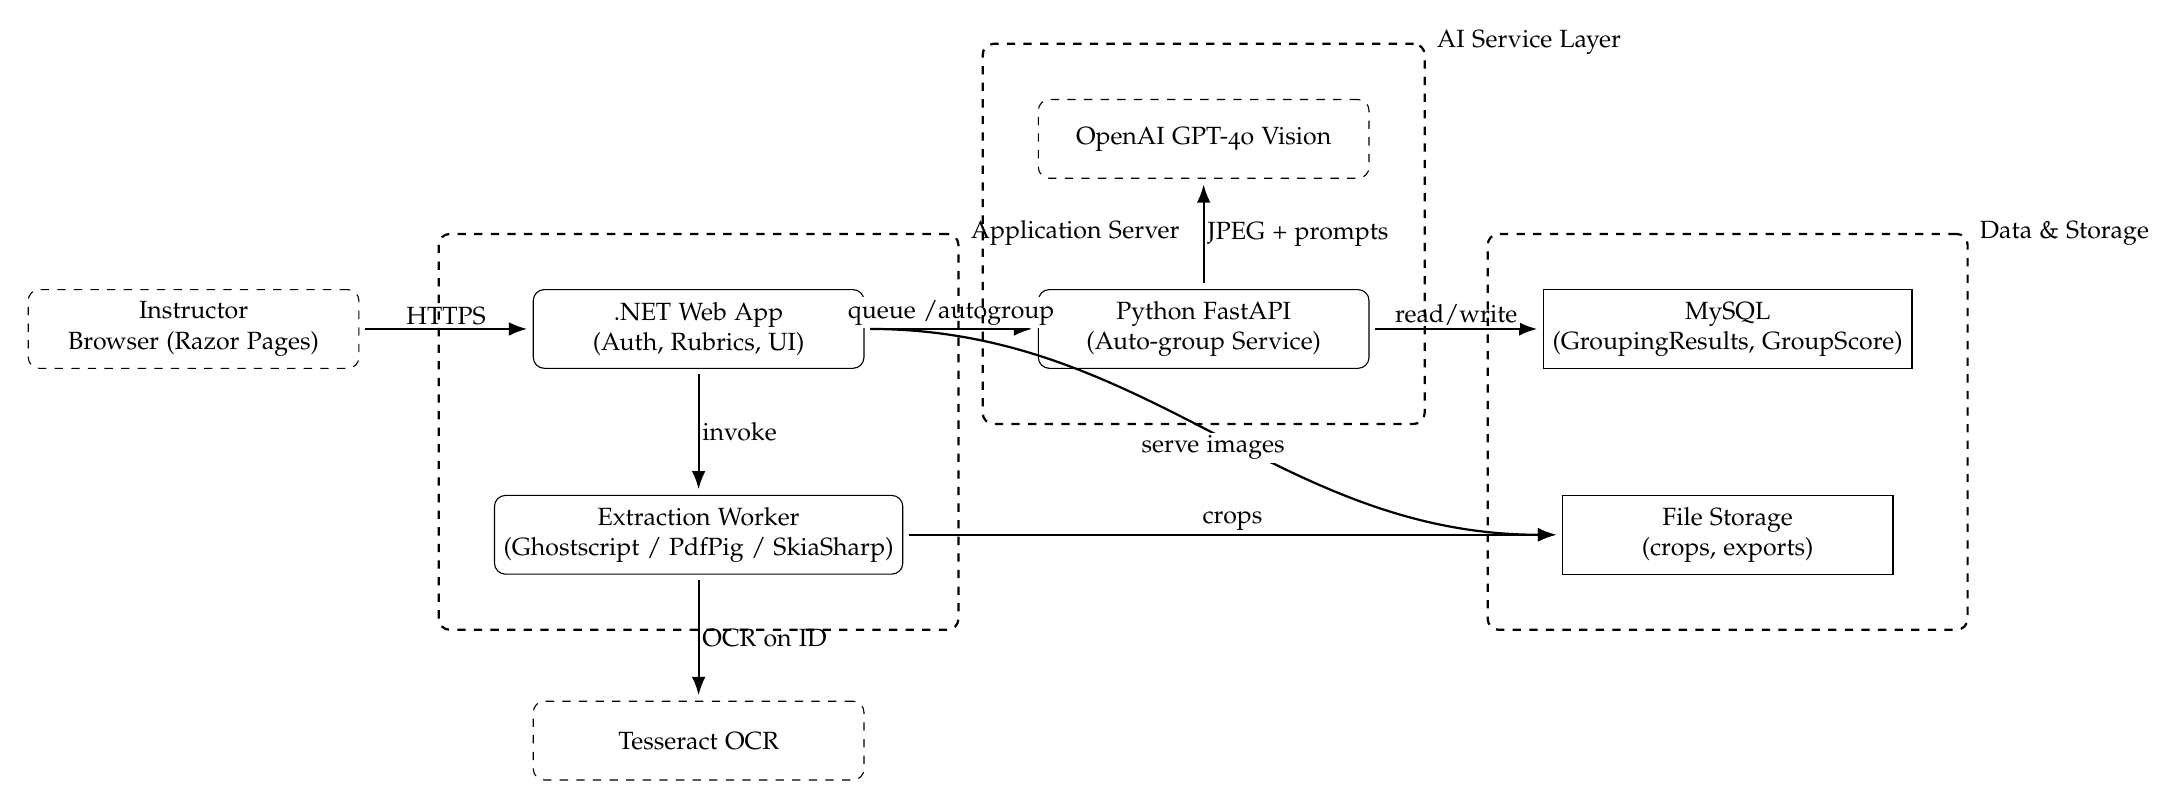
\begin{tikzpicture}[
  font=\small,
  node distance=12mm and 22mm,
  box/.style={draw,rounded corners,align=center,minimum width=42mm,minimum height=10mm,fill=white},
  ext/.style={box,dashed},
  store/.style={draw,align=center,minimum width=42mm,minimum height=10mm,fill=white},
  zone/.style={draw,rounded corners,thick,dashed,inner sep=7mm,fit=#1},
  arrow/.style={-Latex,thick,shorten >=2pt,shorten <=2pt},
  lbl/.style={midway,fill=white,inner sep=1pt}
]

% --- Nodes (grid layout) ---
\node[ext]                            (ui)     {Instructor\\Browser (Razor Pages)};
\node[box,   right=22mm of ui]        (web)    {.NET Web App\\(Auth, Rubrics, UI)};
\node[box,   right=22mm of web]       (api)    {Python FastAPI\\(Auto-group Service)};
\node[store, right=22mm of api]       (db)     {MySQL\\(GroupingResults, GroupScore)};

\node[box,   below=16mm of web]       (worker) {Extraction Worker\\(Ghostscript / PdfPig / SkiaSharp)};
\node[ext,   below=16mm of worker]    (tess)   {Tesseract OCR};
\node[store, below=16mm of db]        (fs)     {File Storage\\(crops, exports)};
\node[ext,   above=14mm of api]       (openai) {OpenAI GPT-4o Vision};

% --- Flows (labels sit on white so they don't collide) ---
\draw[arrow] (ui)  -- node[lbl,above]{HTTPS} (web);
\draw[arrow] (web) -- node[lbl,above]{queue /autogroup} (api);
\draw[arrow] (api) -- node[lbl,above]{read/write} (db);
\draw[arrow] (api) -- node[lbl,right]{JPEG + prompts} (openai);

\draw[arrow] (web)    -- node[lbl,right]{invoke} (worker);
\draw[arrow] (worker) -- node[lbl,right]{OCR on ID} (tess);

\draw[arrow] (worker) -- node[lbl,above]{crops} (fs.west);
\draw[arrow] (web.east) to[out=0,in=180] node[lbl,below]{serve images} (fs.west);

% (Optional) If you *must* show direct app DB access, uncomment:
% \draw[arrow] (web) to[out=-10,in=180] node[lbl,above]{RW} (db.west);

% --- Zones (moved out a bit) ---
\node[zone={(web) (worker)}] (zoneapp) {};
\node[anchor=west,fill=white,inner sep=1pt]
  at ([xshift=1mm]zoneapp.north east) {Application Server};

\node[zone={(api) (openai)}] (zoneai) {};
\node[anchor=west,fill=white,inner sep=1pt]
  at ([xshift=1mm]zoneai.north east) {AI Service Layer};

\node[zone={(db) (fs)}] (zonedata) {};
\node[anchor=west,fill=white,inner sep=1pt]
  at ([xshift=1mm]zonedata.north east) {Data \& Storage};
\end{tikzpicture}
}
  \caption{High-level components and data flow.}
  \label{fig:architecture}
\end{figure}

\section{Sequence of Operations}
An instructor initiates grouping from the web UI by selecting a question and confirming its configuration (maximum points, rubric, and the set of per-answer image paths). The browser submits this intent to the web app, which records a new job and enqueues a request to the FastAPI microservice at \texttt{/autogroup}. In parallel or beforehand (depending on question state), the extraction worker renders the relevant PDF pages with Ghostscript, enumerates answer regions via PdfPig, and uses SkiaSharp to crop each region to PNG. Lightweight OCR with Tesseract runs only on identifying fields (e.g., cover-page name/ID boxes) to support later reconciliation; the content of answers themselves is not OCRed for grouping. All crops are written to the file store under stable, human-inspectable paths, and the web app exposes read-only URLs so the UI can preview exactly what will be grouped.

Upon receiving an \texttt{/autogroup} task, the FastAPI service prepares the model payload. Each PNG crop is converted to JPEG at a target quality of 50 to reduce bandwidth and context size while preserving legibility for short answers. The service computes a token budget using a 50\% downscale heuristic that caps the number of pixels sent per image; if the source crop exceeds that budget, it is downsampled while maintaining aspect ratio. The prompt attaches each image with \texttt{detail:auto} and instructs the model to propose clusters of semantically similar answers. The prompt also requests that low-confidence or outlier responses be flagged for an \emph{Ungrouped} bucket.

GPT-4o Vision returns candidate clusters that the service further \emph{shapes} before persistence. Each cluster receives a stable UUID so subsequent UI edits (rename, merge, split) can be tracked independently of order. Neutral descriptions are standardized (e.g., using a canonical exemplar from the cluster) and very small clusters are folded into \emph{Ungrouped} based on a configurable minimum size. Optionally, if embeddings are available, near-duplicate microclusters are merged with a conservative similarity threshold to avoid over-fragmentation. The shaped result---including cluster membership, labels, and an audit of any collapsed/ungrouped items---is written to MySQL as one row per question with a foreign key to the job.

While the job runs, the UI polls \texttt{/status/\{job\_id\}} with backoff to avoid excessive load. When the job is \texttt{Complete}, the browser fetches the grouped payload and renders cluster cards with thumbnails backed by the file store. Instructors may rename clusters, reassign individual answers, or merge/split clusters as needed; those edits are persisted incrementally. When grading begins, the UI ties rubric criteria and maximum points to each cluster, enabling a single grading action to fan out to all member answers. Final scores are written through to the \texttt{GroupingResults} and \texttt{GroupScore} tables. The complete message choreography for this workflow is shown in the sequence diagram in Figure~\ref{fig:sequence}.

\begin{figure}[htb]
  \centering
  % sequence-autogroup.tikz  — compact, tidy layout that fits on the page
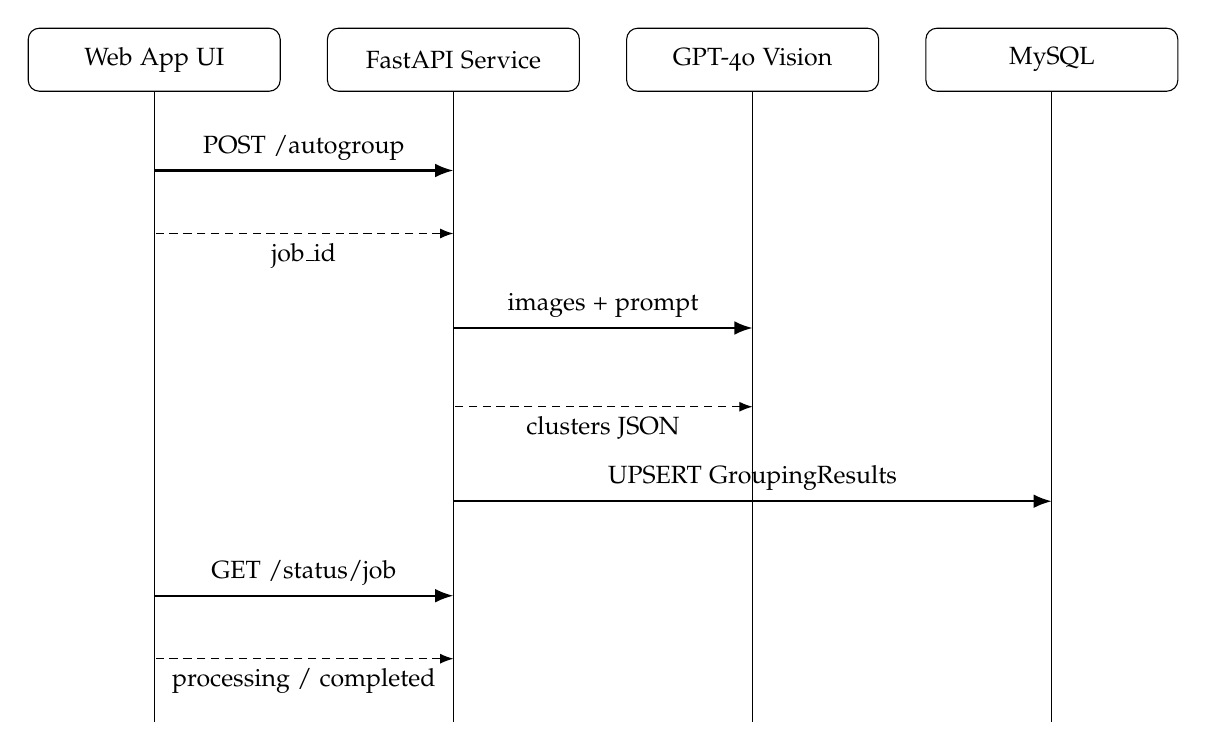
\begin{tikzpicture}[
  font=\small,
  lifeline/.style={draw,rounded corners,align=center,minimum width=32mm,minimum height=8mm,fill=white},
  msg/.style={-Latex,thick},
  ret/.style={Latex-,densely dashed}
]
% fixed spacing so it stays inside \textwidth
\def\xsep{38mm}
\def\H{80mm}

% lifeline headers
\node[lifeline] (ui)  at (0,0)               {Web App UI};
\node[lifeline] (api) at (\xsep,0)           {FastAPI Service};
\node[lifeline] (gpt) at ({2*\xsep},0)       {GPT-4o Vision};
\node[lifeline] (db)  at ({3*\xsep},0)       {MySQL};

% vertical lifelines
\foreach \n in {ui,api,gpt,db} \draw (\n.south) -- ++(0,-\H);

% helpers (avoid repeated coordinate math)
\newcommand{\msg}[5][.5]{%% normal call
  \path (#2.south) ++(0,-#3) coordinate (mstart#3);
  \path (#4.south |- mstart#3) coordinate (mend#3);
  \draw[msg] (mstart#3) -- (mend#3) node[pos=#1,above]{#5};}
\newcommand{\ret}[5][.5]{%% dashed return
  \path (#2.south) ++(0,-#3) coordinate (rstart#3);
  \path (#4.south |- rstart#3) coordinate (rend#3);
  \draw[ret] (rstart#3) -- (rend#3) node[pos=#1,below]{#5};}

% messages — y positions staggered so labels never collide
\msg{ui}{10mm}{api}{POST /autogroup}
\ret{api}{18mm}{ui}{job\_id}

\msg{api}{30mm}{gpt}{images + prompt}
\ret{gpt}{40mm}{api}{clusters JSON}

\msg{api}{52mm}{db}{UPSERT GroupingResults}

\msg{ui}{64mm}{api}{GET /status/{job}}
\ret{api}{72mm}{ui}{processing / completed}
\end{tikzpicture}
  \caption{Sequence for an auto-grouping job.}
  \label{fig:sequence}
\end{figure}

\section{Instructor-Facing UI Snapshots}
This section highlights the key instructor workflows with inline references to the corresponding UI figures: assignment creation (Figure~\ref{fig:assignment-creation}), the course assignments overview (Figure~\ref{fig:course-page}), the shared region-cropping tool (Figure~\ref{fig:ui-crops}), and the auto-grouping interface (Figure~\ref{fig:ui-grouping}).

\paragraph{Assignment creation.}
Instructors configure the submission layout (\emph{filled-form} vs.\ \emph{free-form}), directions, and dates. As shown in Figure~\ref{fig:assignment-creation}, the authoring adapts to the chosen layout: 
\begin{compactitem}
  \item \textbf{Free-form:} the instructor enters \emph{only} the question labels (e.g., \texttt{Q1}, \texttt{Q2a}) and max points per question. No region editor is shown here because students will upload a PDF and \emph{define their own answer regions} in the next step (see also the cropping widget in Figure~\ref{fig:ui-crops}).
  \item \textbf{Filled-form:} in addition to questions/points, the instructor binds an exam template and draws the \emph{identity} and \emph{answer} regions once. Those regions are then used to crop all submissions automatically (the same widget used here is illustrated in Figure~\ref{fig:ui-crops}).
\end{compactitem}

\begin{figure}[htb]
  \centering
  \IfFileExists{images/assignment-creation.png}{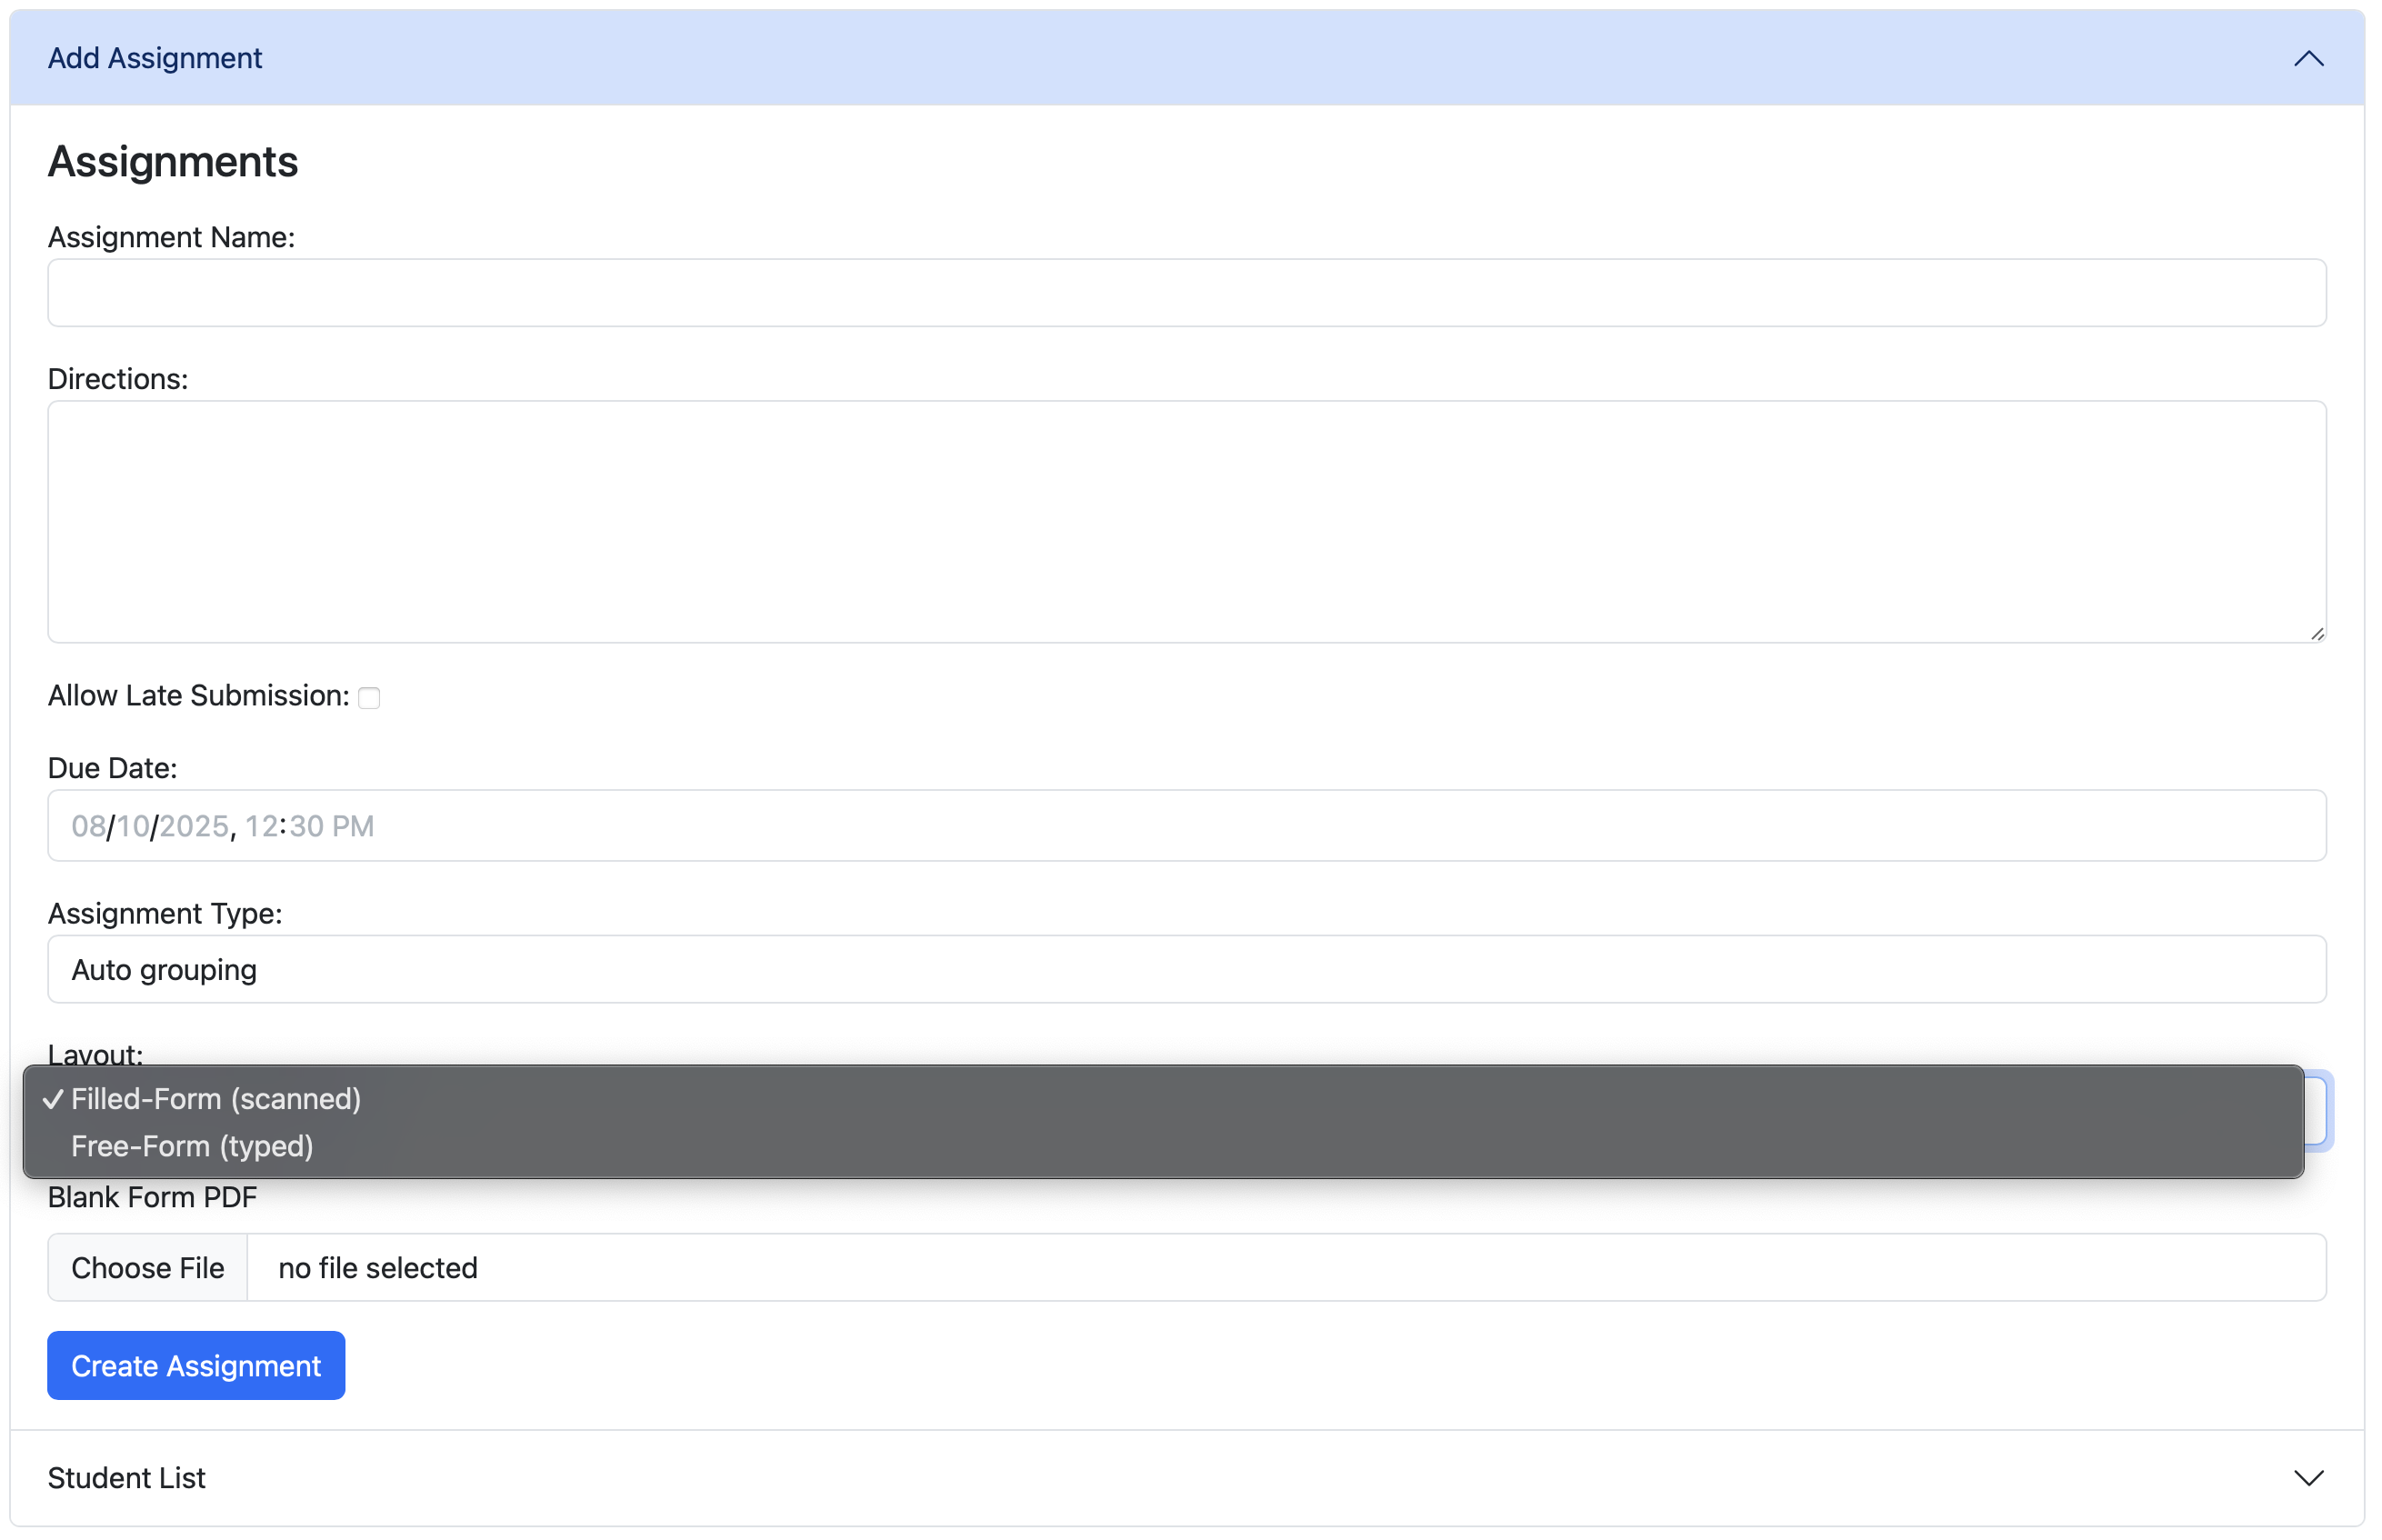
\includegraphics[width=.92\textwidth]{assignment-creation.png}}{%
    \fbox{\parbox{.92\textwidth}{Placeholder: add \texttt{images/assignment-creation.png}}}}
  \caption{Assignment creation form. For free-form, authors enter questions and points only; for filled-form, authors also define identity/answer regions against a template.}
  \label{fig:assignment-creation}
\end{figure}

\paragraph{Course assignments page.}
The course view summarizes assignment state (open/closed, submissions, grading progress) and links to grouping/grading. Figure~\ref{fig:course-page} shows status indicators and quick actions that guide instructors into grouping (Figure~\ref{fig:ui-grouping}) or back to the region editor (Figure~\ref{fig:ui-crops}) if setup needs adjustment.

\begin{figure}[htb]
  \centering
  \IfFileExists{images/course-page.png}{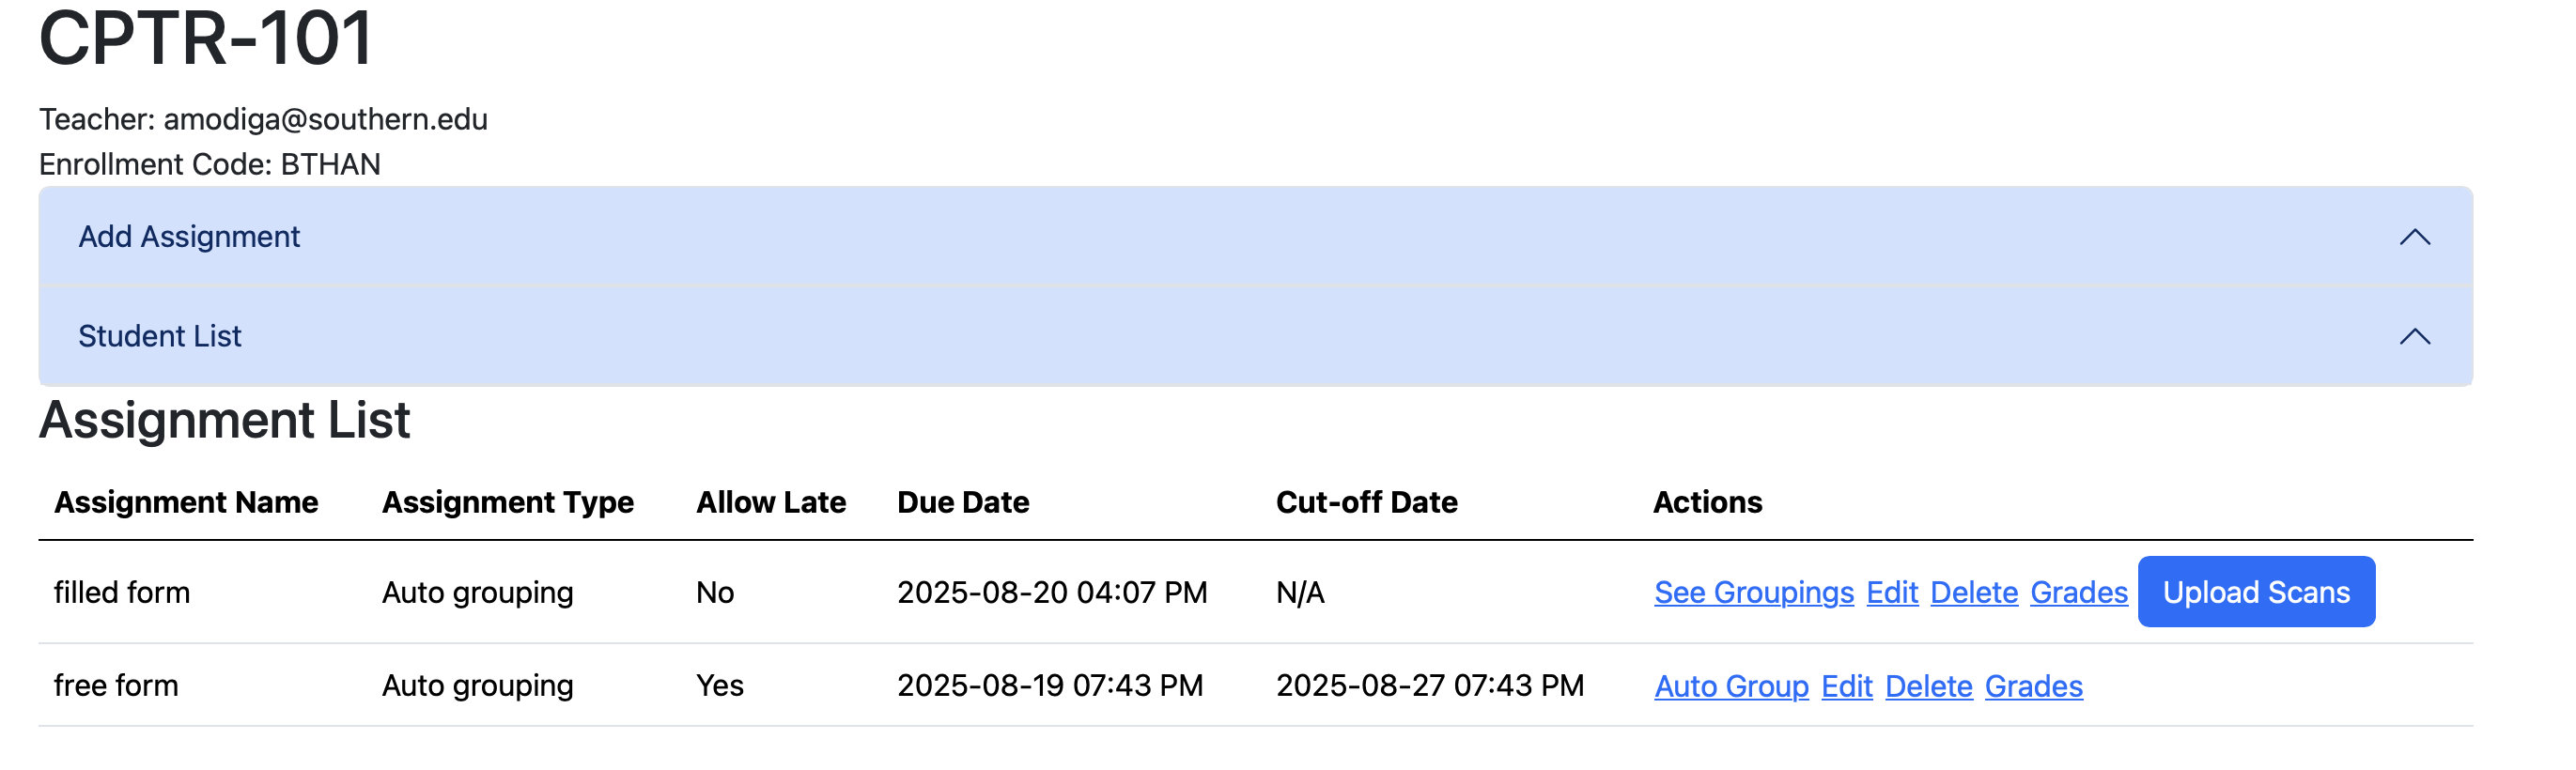
\includegraphics[width=.92\textwidth]{course-page.png}}{%
    \fbox{\parbox{.92\textwidth}{Placeholder: add \texttt{images/course-page.png}}}}
  \caption{Course assignments overview with status indicators and quick actions.}
  \label{fig:course-page}
\end{figure}

\paragraph{Region extraction (shared tool).}
The same cropping widget is used to verify identity/answer regions for filled-form scans and, in free-form flows, to let students mark their own answer areas. Figure~\ref{fig:ui-crops} depicts the shared tool; the resulting crops flow directly into the grouping experience shown in Figure~\ref{fig:ui-grouping}.

\begin{figure}[htb]
  \centering
  \IfFileExists{images/region-extraction.png}{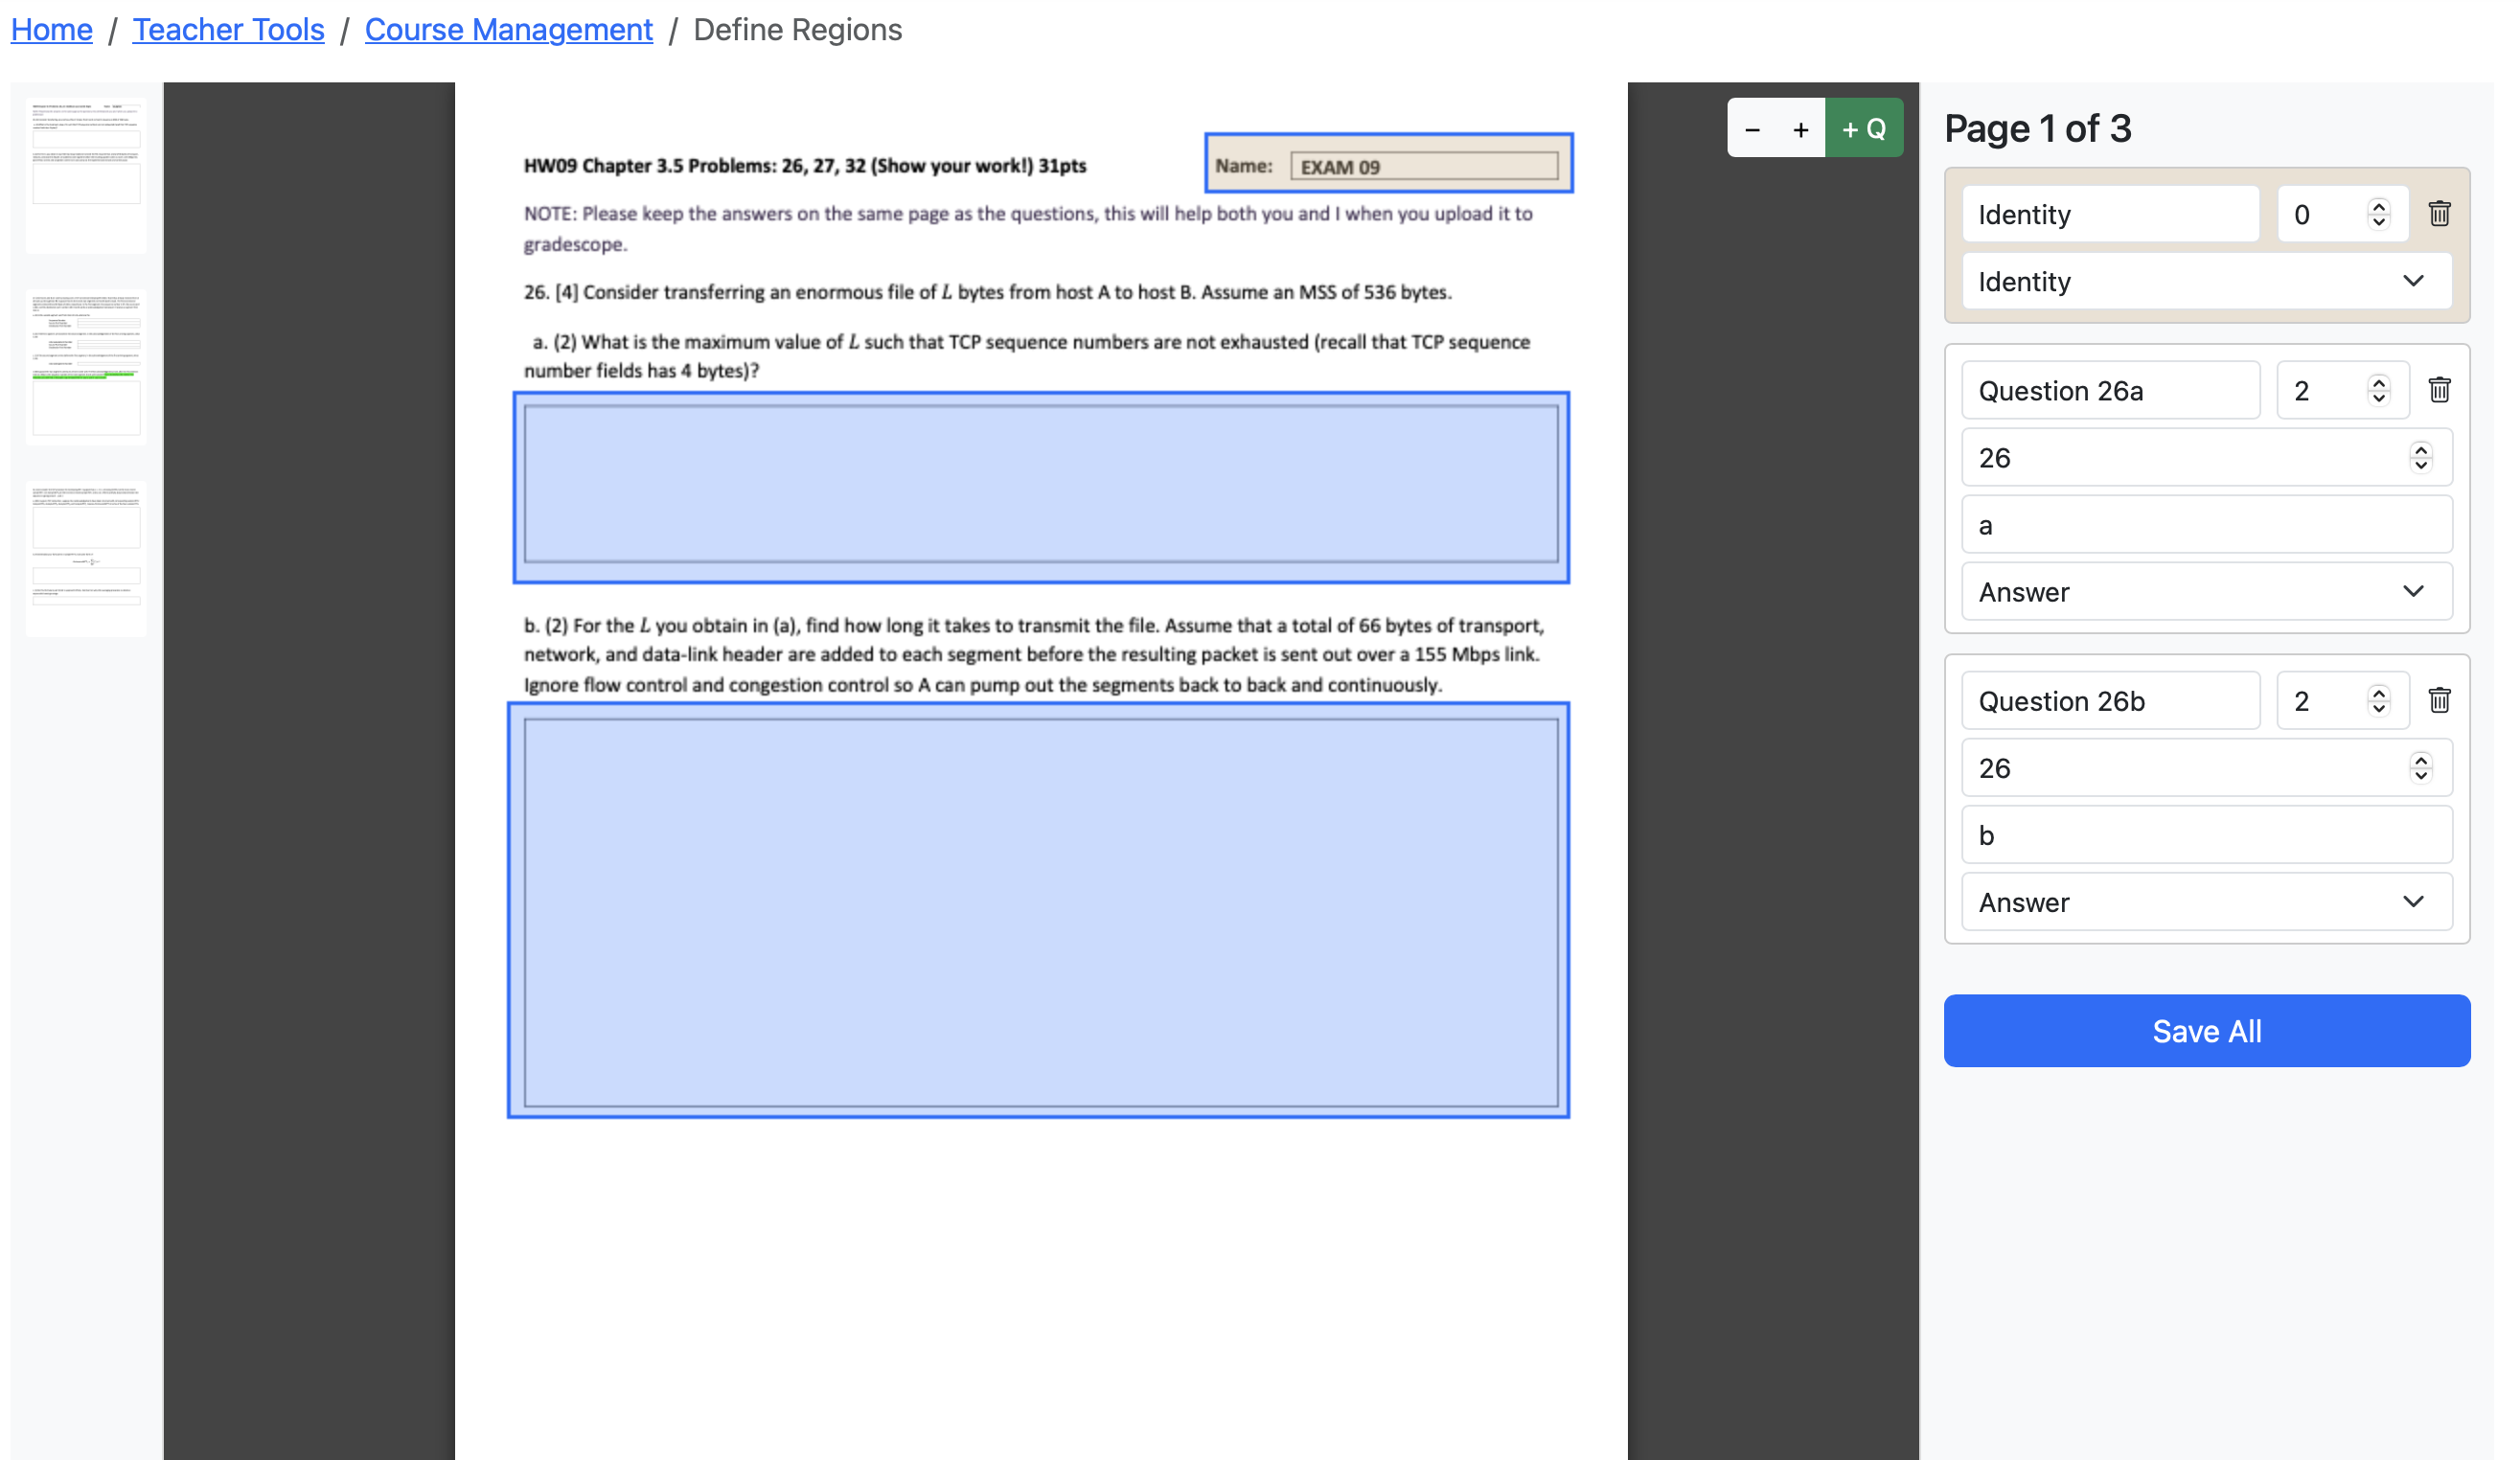
\includegraphics[width=.92\textwidth]{region-extraction.png}}{%
    \fbox{\parbox{.92\textwidth}{Placeholder: add \texttt{images/region-extraction.png}}}}
  \caption{Region cropping widget used in two contexts: (i) instructor verification for filled-form scans and (ii) student free-form ``mark your answers'' flow.}
  \label{fig:ui-crops}
\end{figure}

\paragraph{Auto-grouping UI.}
After crops are generated, the grouping page proposes semantic clusters; instructors can merge/split groups, move items, and apply rubric items per group. Figure~\ref{fig:ui-grouping} shows the proposed clusters and edit tools; rubric-first grading executed here propagates scores to all members of a cluster.

\begin{figure}[htb]
  \centering
  \IfFileExists{images/grouping-answers.png}{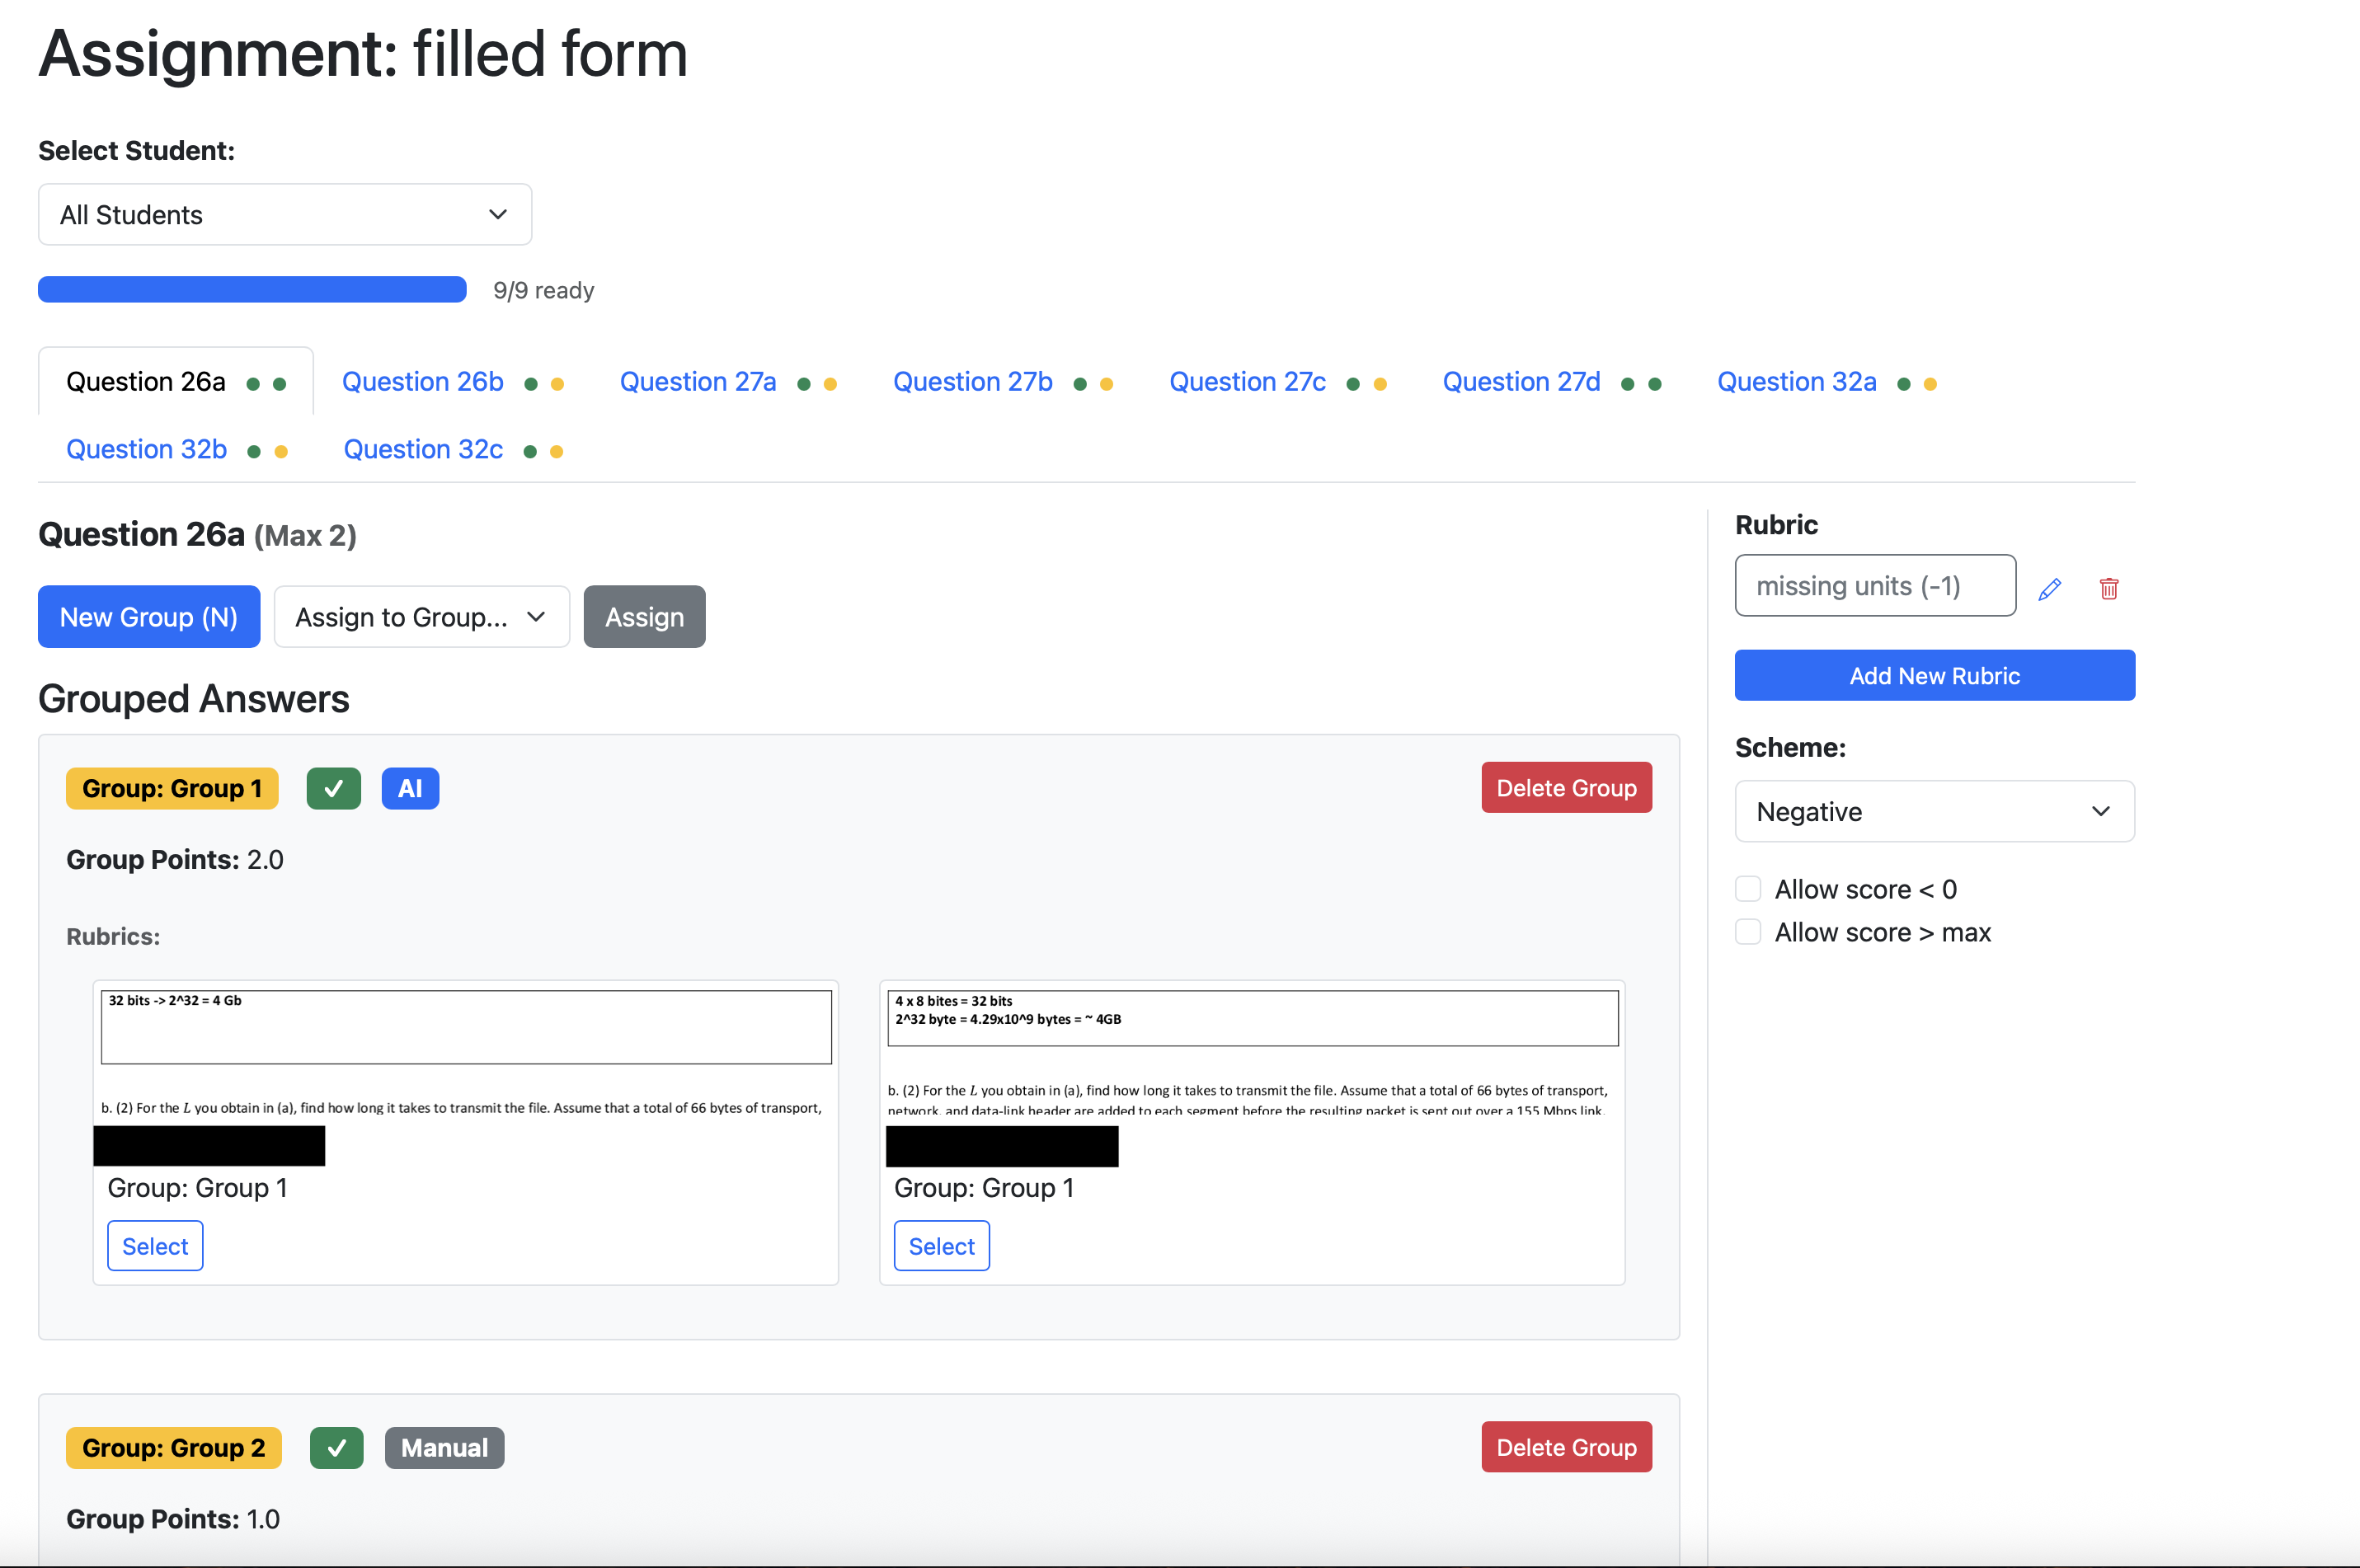
\includegraphics[width=.92\textwidth]{grouping-answers.png}}{%
    \fbox{\parbox{.92\textwidth}{Placeholder: add \texttt{images/grouping-answers.png}}}}
  \caption{Auto-grouping page with proposed clusters, edit tools, and rubric-first grading.}
  \label{fig:ui-grouping}
\end{figure}

\section{Region Extraction and File Lifecycle}
For \textbf{filled-form} assignments, instructors define identity and answer regions once per assignment using the cropping widget (Figure~\ref{fig:ui-crops}); the worker then applies those regions to every scanned booklet and enforces stable filenames (e.g., \texttt{Q27a.png}) for reproducibility and idempotent re-uploads. For \textbf{free-form} assignments, students upload a PDF and mark their own answer regions in the same tool (Figure~\ref{fig:ui-crops}); the saved boxes are used to generate per-question crops that populate the grouping interface (Figure~\ref{fig:ui-grouping}) for review and rubric-first grading. Debug images are suppressed outside development builds. Re-uploads replace prior crops and metadata to avoid stale data, and the updated crops reappear in the grouping view (Figure~\ref{fig:ui-grouping}) so that any instructor edits remain aligned with the latest artifacts.

\section{Identity Assignment}
Filled-form batches use Tesseract~\cite{tesseract} to extract roster identifiers from the pre-defined \emph{identity} region (see Figure~\ref{fig:ui-crops}). Low-confidence or malformed results are flagged for manual resolution with a roster pick-list and a thumbnail preview. Free-form uploads are tied to the uploader’s account; therefore no OCR is needed. Identity OCR is used only for roster linkage—semantic grouping operates directly on cropped answer images (Section~\ref{chap:solution}, Figures~\ref{fig:architecture} and~\ref{fig:sequence}).

\section{Grouping Heuristics}
We instruct the model to produce \emph{fewer, larger clusters}, to route unreadable/singletons into \emph{Ungrouped}, and to emit neutral descriptions (\enquote{Group 1}, \enquote{Group 2}). Tiny groups under a threshold are collapsed into \emph{Ungrouped}. Groups are sequentially re-numbered for clarity. All prompts and model versions are archived with the \texttt{job\_id}.

\section{Data Model}
Auto-grouping results are persisted as a \emph{single row per question}, providing a denormalized snapshot that the UI can load quickly after the workflow in Figure~\ref{fig:sequence} and during review in Figure~\ref{fig:ui-grouping}. As summarized in Table~\ref{tab:groupingresults}, the JSON payload \texttt{GroupData} holds the proposed/edited clusters (neutral labels, membership, per-group points/flags), while \texttt{ScoringScheme} and the boolean guards (\texttt{AllowBelowZero}, \texttt{AllowAboveMax}) control rubric arithmetic. \texttt{CreatedAt}/\texttt{UpdatedAt} provide auditability. In practice, there is at most one record per \texttt{(AssignmentId, AssignmentQuestionId)}; edits typically mutate \texttt{GroupData} and bump \texttt{UpdatedAt}.

\begin{table}[H]
  \centering
  \caption{Key table: \texttt{GroupingResults}.}
  \label{tab:groupingresults}
  \setlength\tabcolsep{6pt}
  \renewcommand{\arraystretch}{1.2}
  \footnotesize
  \begin{tabularx}{\textwidth}{@{}L{4.3cm}L{2.8cm}Y@{}}
    \toprule
    \textbf{Column} & \textbf{Type} & \textbf{Notes} \\
    \midrule
    Id & INT (PK) & Surrogate primary key. \\
    AssignmentId & INT (FK) & Links to the assignment entity. \\
    AssignmentQuestionId & INT (FK) & Equals \texttt{template\_region\_id} sent by client. \\
    GroupData & JSON & Array of groups with files, description, \texttt{is\_correct}, \texttt{points}. \\
    ScoringScheme & VARCHAR(32) & Default \texttt{"Negative"}. \\
    AllowBelowZero & TINYINT(1) & Boolean. \\
    AllowAboveMax & TINYINT(1) & Boolean. \\
    CreatedAt & DATETIME & UTC created timestamp. \\
    UpdatedAt & DATETIME NULL & UTC last update; nullable. \\
    \bottomrule
  \end{tabularx}
\end{table}

\paragraph{Prompting \& JSON schema.}
The service uses concise grouping rules (favor fewer, larger clusters; neutral labels; unreadable/singletons $\rightarrow$ \emph{Ungrouped}). Prompts and model/version are archived with each \texttt{job\_id}. The model returns JSON in the following abbreviated form:
\begin{lstlisting}[language=json]
{
  "groups": [
    {
      "group_id": "uuid",
      "files": [
        {
          "file_path": "...",
          "user_id": "...",
          "template_region_id": "...",
          "question_label": "...",
          "content_type": "image/jpeg",
          "user_name": "..."
        }
      ],
      "description": "Group 1",
      "is_correct": true | false | null,
      "points": 5.0
    }
  ]
}
\end{lstlisting}

\section{Token Budget, Cost \& Rate Limiting}
For an image of width $w$ and height $h$, the service estimates tokens after a 50\% downscale: $w' = \lfloor w/2 \rfloor$, $h' = \lfloor h/2 \rfloor$. The number of 512$\times$512 tiles is $T=\lceil w'/512 \rceil\cdot\lceil h'/512 \rceil$, and the cost estimate is $85 + 170\,T$ tokens/image. Batches exceeding a threshold are split. On rate limits, the client retries up to 10 times with exponential backoff. For a representative $768\times 768$ downscaled image ($T=3$), the estimate is $\sim595$ tokens/image.

\section{Integration with ASP.NET}
The web app calls \texttt{QueueAutoGroupAsync} (server) to POST to \texttt{/autogroup}, records a \texttt{GroupingJob}, and renders a progress UI that polls \texttt{/status/\{job\_id\}}; when the background job completes, the page automatically refreshes into the results view. Subsequent instructor actions (save groups, apply/remove rubric items, scoring method toggles) are persisted in the relational database and mirrored in a \texttt{GroupScore} table; a background grade recalculator keeps submission grades in sync.

\section{Service Isolation \& Network Security}
In production, the FastAPI auto-grouping service runs inside the same Docker Compose stack on a private bridge network and is not published to the host (container uses \texttt{expose} only—no \texttt{ports} mapping). As a result, \texttt{/autogroup} and related endpoints are reachable only from the web app over internal service DNS (e.g., \texttt{http://autogroup:8000/...}); the browser never talks to the service directly. Compose-level network isolation and host firewall rules prevent external ingress to the service container.


\section{Student-Facing Assignment UI}
Students reach an assignment-specific page that adapts to the configured layout:

\paragraph{Filled-form (read-only).}
Students cannot upload; they can download the submitted booklet (when present) and view the grade once posted. The page shows \texttt{Directions} and a simple status panel.

\paragraph{Free-form (student upload).}
Students upload a single PDF, then are routed to a \texttt{DefineAnswerRegions} step to mark answer boxes. When submissions are open (\texttt{DueDate}/\texttt{AllowLateWork}/\texttt{CutoffDate} enforced via \texttt{CanSubmit()}), they can resubmit; otherwise the page displays a \enquote{Resubmissions have closed} notice. \emph{Note:} The region-marking widget for free-form uploads reuses the same cropping interface shown in \Cref{fig:ui-crops}; we avoid duplicating the screenshot here.

\begin{figure}[htb]
  \centering
  \IfFileExists{images/student-assignment.png}{
\includegraphics[width=.92\textwidth]{student-assignment.png}}{%
    \fbox{\parbox{.92\textwidth}{Placeholder: add \texttt{images/student-assignment.png}}}}
  \caption{Student assignment page: layout indicator (filled vs.\ free-form), PDF upload (free-form only), download of submitted file, and grade display.}
  \label{fig:ui-student}
\end{figure}

\section{Rubrics and Grading UX}
While grading a group, instructors select and apply rubric items; zoom/pan is supported where available. Changing a rubric value propagates to all affected answers. The Question tab shows review status: each group displays a status badge (\enquote{Graded} or \enquote{Needs grading}). Instructors can either apply at least one rubric item or, if none are needed, click \texttt{Save All Groups for Question} to mark the question as reviewed.

\section{Security \& Privacy}
We minimize student-data exposure by limiting OCR strictly to identity regions (therefore no OCR is needed on answers), sending only per-answer image crops—without student names—to the vision model for grouping, and confining operations to authenticated instructor actions with role-appropriate permissions. Only course roster identifiers and per-answer images are processed; no plaintext student content is transmitted for grouping. All reads and writes are logged for auditability, and the design follows least-privilege access control consistent with FERPA expectations~\cite{FERPA1974}. To safeguard fairness, we monitor for potential bias by auditing cluster assignments across demographic-neutral cohorts and preserve human authority through full instructor override mechanisms for grouping and grading.

\section{Threat Model \& Data Handling}
This section details how identities, images, and grouping results are protected throughout the workflow in Figure~\ref{fig:sequence} and during review in Figure~\ref{fig:ui-grouping}. For a concise summary, see Table~\ref{tab:threats} at the end of this section.

\paragraph{Roles and access scope.}
\textbf{Students} may upload their own work and view only their own grades; they cannot view other students’ submissions, crops, or groupings. \textbf{Instructors} (course owners/graders) can access assignments, submissions, identity crops for their course, grouping results, and grading tools; their access is scoped per course via ACLs. \textbf{Administrators} handle configuration and support tasks; by policy they do not browse student content unless temporarily granted course-scoped access for incident response.

\paragraph{Unauthorized access.}
\emph{Risk.} A user without rights could read crops, grouping results, or grades. \emph{Mitigation.} Role-based authorization (student/instructor/admin) plus per-course ACLs are enforced at the server for every endpoint that touches identity crops, answer crops, grouping JSON, or grade records. The UI never embeds direct file paths without an authorization check; URLs are resolved through the web app to ensure policy is applied. Audit logs provide a trail of who saw or changed what, enabling both deterrence and post-hoc review.

\paragraph{Model data exposure.}
\emph{Risk.} Personally identifiable information (PII) might be sent to a third-party model. \emph{Mitigation.} Only identity regions contain PII and are processed locally to assign roster IDs. Grouping uses per-answer crops that exclude names and form headers; no student plaintext is transmitted for clustering. Prompts avoid including course/roster metadata, and the shaped outputs (neutral group descriptions, UUIDs) intentionally carry no PII.

\paragraph{Prompt injection and model influence.}
\emph{Risk.} Crafted markings within an answer image attempt to steer the model (e.g., \enquote{put all answers into one group}). \emph{Mitigation.} The service uses fixed, server-side prompts and normalizes model responses before persistence: clusters receive stable UUIDs and neutral labels; tiny or low-confidence clusters are folded into \emph{Ungrouped}. Instructors retain full control to rename, merge, split, or reassign items, ensuring human oversight dominates over model suggestions.

\paragraph{Data retention and scope.}
\emph{Risk.} Retaining artifacts longer than needed increases exposure. \emph{Mitigation.} Identity crops and derived answer crops follow course-level retention settings; exports are versioned, and re-uploads purge and regenerate crops to avoid drift. Grouping JSON (\texttt{GroupData}) stores neutral labels and membership only; it excludes raw identity text. Retention and deletion actions are logged.

\begin{table}[H]\centering
\caption{Abbreviated threat model and mitigations}\label{tab:threats}
\begin{tabularx}{\textwidth}{@{}p{3.8cm}Xp{4.6cm}@{}}
\toprule
\textbf{Threat} & \textbf{Risk} & \textbf{Mitigation} \\
\midrule
Unauthorized access & Disclosure of student data & Role-based auth; per-course ACLs; object-level checks; audit logs \\
Model data exposure & PII leakage to third party & PII limited to local identity OCR; answer crops exclude names; neutral outputs \\
Prompt injection & Manipulated grouping suggestions & Server-side prompts; normalize outputs; full instructor override \\
Data retention & Oversharing over time & Course retention settings; purge-on-reupload; logged deletions/exports \\
\bottomrule
\end{tabularx}
\end{table}


\section{Limitations \& Risks}
\begin{compactitem}
  \item \textbf{Generalization:} Prompts tuned on one course may not transfer perfectly to other subjects; mitigated by neutral labels and editable groups.
  \item \textbf{Model drift:} Vision model updates can shift behavior; we pin model/version and archive prompts with run IDs.
  \item \textbf{Edge cases:} Faint pencil, skew, or multiple answers in one crop reduce grouping confidence; flagged to \emph{Ungrouped}.
  \item \textbf{Human factors:} Instructor trust varies; we look to why/where groups changed and keep full override tools.
\end{compactitem}

% --------------------------------------------------------------------------------
\chapter{Testing and Evidence}\label{chap:evalplan}

\section{Objectives}
We provide concise, visual evidence that the system:
(i) processes submissions end-to-end,
(ii) groups answer \emph{images} by semantic similarity (no answer OCR; therefore none is needed),
(iii) isolates outliers for review,
(iv) applies rubrics and propagates score changes consistently, and
(v) supports clipboard-based grade transfer (\emph{Copy Table}) into external systems.

\section{Test Data}
A small gold-labeled set (12–20 pages) mixing typed and handwritten responses. Known-correct exemplars are used only to \emph{interpret} cluster coherence; the system does not OCR answer content for grouping.

\section{Tests \& Evidence}
\textbf{A. Basic Flow.} Upload~$\rightarrow$ process~$\rightarrow$ results; rubric application updates totals.  
\emph{Evidence:} one multi-panel figure combining upload/process, results view, and rubric before/after (Figure~\ref{fig:basic-flow}).

\textbf{B. Vision-Based Semantic Recognition (No Answer OCR).}
GPT-4o Vision groups answer \emph{images} by meaning.  
\emph{Evidence:} a compact figure with (a) Cluster~A gallery (similar idea), (b) Cluster~B gallery (different idea), and (c) Outliers gallery (heterogeneous/suspect) (Figure~\ref{fig:vision-groups}).

\textbf{C. Rubric Propagation \& Clipboard Interop.}
Totals update after a rubric edit; the on-screen grade table can be copied to the clipboard and pasted into an LMS/spreadsheet.  
\emph{Evidence:} a figure showing the \emph{Copy Table} UI and the pasted result (Figure~\ref{fig:copy-table}).

\section{UI Verification Checklist (Feature Presence)}
This checklist is completed once per build to verify that all expected UI elements and flows are present. Evaluators mark \texttt{[X]} or leave blank; notes capture anything missing or confusing.

\begin{table}[H]\centering
\caption{UI checklist for instructor workflow (presence, not preference).}\label{tab:ui-checklist}
\begin{tabularx}{\textwidth}{@{}p{6.7cm}p{1.2cm}X@{}}
\toprule
\textbf{Item} & \textbf{OK} & \textbf{Notes} \\
\midrule
Assignment creation (free-form + filled-form options) & [ ] &  \\
Template binding and identity/answer region editor (filled-form) & [ ] &  \\
Student upload flow; processing status/notifications & [ ] &  \\
Grouping view with clusters + \emph{Ungrouped} bucket & [ ] &  \\
Cluster edit tools (rename, merge, split, reassign) & [ ] &  \\
Rubric panel; apply/remove rubric items per group & [ ] &  \\
Totals update immediately after rubric edit & [ ] &  \\
Copyable grade table (\emph{Copy Table}) & [ ] &  \\
Pasted table preserves rows/columns in target app & [ ] &  \\
Audit-friendly identifiers (assignment, question, job id) visible & [ ] &  \\
\bottomrule
\end{tabularx}
\end{table}

\paragraph{Suggested UI screenshots (placeholders).}
\begin{figure}[H]
  \centering
  \begin{subfigure}{0.49\linewidth}
    \MaybeImage[0.99\linewidth]{basic_upload.png}
    \caption{Upload \& processing}
  \end{subfigure}\hfill
  \begin{subfigure}{0.49\linewidth}
    \MaybeImage[0.99\linewidth]{basic_results.png}
    \caption{Results view}
  \end{subfigure}

  \vspace{0.5em}
  \begin{subfigure}{0.49\linewidth}
    \MaybeImage[0.99\linewidth]{rubric_before.png}
    \caption{Rubric before}
  \end{subfigure}\hfill
  \begin{subfigure}{0.49\linewidth}
    \MaybeImage[0.99\linewidth]{rubric_after.png}
    \caption{Rubric after (totals updated)}
  \end{subfigure}
  \caption{End-to-end processing and rubric application.}
  \label{fig:basic-flow}
\end{figure}

\section{UX Design Evaluation (Questionnaire)}
\textbf{Participants.} 3–6 instructors/TAs familiar with grading.  
\textbf{Scope.} Design/readability only (layout, labels, hierarchy, contrast, discoverability)—\emph{not} speed or task timing.

\paragraph{Likert (1–5) items used.}
\begin{compactenum}
  \item The layout feels clean and uncluttered.
  \item Text is legible without zooming; font sizes are appropriate.
  \item Color/contrast makes content easy to read (including low-light).
  \item Visual hierarchy makes the primary actions obvious.
  \item Labels and terminology are clear and unambiguous.
  \item Icons and buttons are self-explanatory or clearly labeled.
  \item Whitespace/spacing helps me scan and find things quickly.
  \item Clusters are visually distinguishable from each other.
  \item Thumbnails are large and crisp enough to compare answers.
  \item Edit affordances (rename/merge/split/reassign) are easy to find.
  \item The rubric panel is easy to locate and interpret.
  \item Score changes and totals are clearly indicated.
  \item Empty/error states are understandable and instructive.
  \item Loading/progress indicators are clear and non-distracting.
  \item Keyboard focus is visible and navigation feels predictable.
  \item Color is not the only cue (labels/icons also indicate meaning).
  \item Overall, the design feels easy to read and understand.
\end{compactenum}
\textbf{Free-response prompts.}  
(1) What was hard to read, notice, or understand?  
(2) One UI element you would improve and how.  
(3) Accessibility notes: contrast, text size, color cues, keyboard focus, screen readers.

\section{Model Grouping Accuracy (10-Student Run)}
\textbf{Setup.} Run one assignment with $\sim$10 students. For a single question, create a \emph{gold} clustering by manually assigning each answer crop to a semantic group (visual meaning).  
\textbf{Prediction.} Record the model’s shaped output (cluster IDs, memberships, \emph{Ungrouped}).  
\textbf{Metrics.} Report B-Cubed Precision/Recall/F1, Pairwise F1, \emph{Ungrouped Precision}, and Coverage.

\begin{table}[H]\centering
\caption{Clustering metrics for one question (10-student run; fill with results).}\label{tab:cluster-metrics}
\begin{tabularx}{\textwidth}{@{}lcccccc@{}}
\toprule
\textbf{Question} & \textbf{B3-P} & \textbf{B3-R} & \textbf{B3-F1} & \textbf{Pair-F1} & \textbf{Ungrp.\ P} & \textbf{Coverage} \\
\midrule
Q\# (label) & 0.00 & 0.00 & 0.00 & 0.00 & 0.00 & 0.00 \\
\bottomrule
\end{tabularx}
\end{table}

\section{Clipboard Interoperability (Evidence)}
\begin{figure}[H]
  \centering
  \begin{subfigure}{0.6\linewidth}
    \MaybeImage[0.99\linewidth]{copy_table.png}
    \caption{Copyable grade table in the app}
  \end{subfigure}

  \vspace{0.5em}
  \begin{subfigure}{0.6\linewidth}
    \MaybeImage[0.99\linewidth]{paste_example.png}
    \caption{Pasted result in external tool}
  \end{subfigure}
  \caption{Clipboard-based grade transfer using \emph{Copy Table}.}
  \label{fig:copy-table}
\end{figure}

% --------------------------------------------------------------------------------
\chapter{Results}\label{chap:results}

\section{UI Verification}
Table~\ref{tab:ui-checklist} was completed for the evaluated build. All required UI elements and flows were present unless noted in the checklist’s \emph{Notes} column. Figure~\ref{fig:basic-flow} illustrates the end-to-end flow and rubric propagation.

\section{Vision-Based Semantic Grouping (No Answer OCR)}
The system groups \emph{answer crops} by visual meaning rather than OCR. Figure~\ref{fig:vision-groups} shows two coherent clusters and an outlier set; each tile is a raw crop.

\begin{figure}[H]
  \centering
  \begin{subfigure}{0.32\linewidth}
    \MaybeImage[0.99\linewidth]{cluster_A_gallery.png}
    \caption{Cluster A (same idea)}
  \end{subfigure}\hfill
  \begin{subfigure}{0.32\linewidth}
    \MaybeImage[0.99\linewidth]{cluster_B_gallery.png}
    \caption{Cluster B (different idea)}
  \end{subfigure}\hfill
  \begin{subfigure}{0.32\linewidth}
    \MaybeImage[0.99\linewidth]{cluster_outliers.png}
    \caption{Outliers (mixed/unclear)}
  \end{subfigure}

  \vspace{0.75em}
  \MaybeImage[0.6\linewidth]{grouping_scatter.png}

  \caption{Vision-led semantic grouping from images only: coherent clusters (left, middle) and outliers (right).}
  \label{fig:vision-groups}
\end{figure}

\section{UX Design Outcomes}
Report median and IQR per Likert item (1–5) and summarize key themes from free responses (readability, hierarchy, contrast, discoverability). Highlight any accessibility issues and proposed changes (e.g., increasing contrast on disabled controls).

\section{Model Grouping Metrics}
Populate Table~\ref{tab:cluster-metrics} with measured values for the chosen question(s). Summarize notable errors (e.g., near-duplicate answers split across clusters) and whether \emph{Ungrouped} captured true outliers.

\section{Clipboard Interoperability}
Figure~\ref{fig:copy-table} shows the source grade table and pasted result. Note any differences (e.g., numeric formatting) and remediation steps if needed.

\section{Summary}
Across these tests, we visually confirm end-to-end processing, vision-based semantic grouping with isolated outliers, consistent rubric propagation, and successful clipboard transfer of grades. The UI checklist verifies feature presence; the design-only UX questionnaire gauges readability and clarity; and clustering metrics quantify grouping quality on a 10-student run.


% -------------------------------------------------
\chapter{Conclusion}
\section{Summary of Problem and Goals}
We addressed the effort and inconsistency of grading open-ended work by building an instructor-in-the-loop system that extracts regions, assigns identity via OCR, groups answers with a vision LLM, and enables rubric-first grading with auditability.

\section{Evaluation Summary}
Our visual tests demonstrated end-to-end processing, coherent semantic grouping (no answer OCR), consistent rubric propagation, and reliable clipboard-based grade transfer using \emph{Copy Table}.

\section{Final Outcomes and Deliverables}
We delivered the integrated web app, background services, reproducible prompts/model versions, and a \emph{Copy Table} flow that enables fast pasting of grades into external systems (e.g., LMS/Sheets). Documentation includes an instructor guide and technical deployment notes.

\section{Lessons Learned and Future Work}
\begin{compactitem}
  \item Visual pre-processing (downscale/tiling) mattered more for stability than minor prompt tuning.
  \item Instructors preferred neutral group names and an explicit \emph{Ungrouped} bin.
  \item Future: direct CSV/Excel export in addition to \emph{Copy Table}; domain-tuned prompts for math diagrams; adaptive thresholding for faint pencil; pre-clustering to cut LLM calls; regrade workflow.
\end{compactitem}

% ===================== Appendix =====================
\appendix

\chapter{Configuration and Deployment}\label{app:config}

This appendix captures the minimum configuration to run the system on a fresh machine.
Replace placeholders (the ALL-CAPS bits) with values for your environment.

% Keep code within margins
\lstset{basicstyle=\ttfamily\footnotesize,breaklines=true,columns=fullflexible}

\section{Prerequisites}
\begin{compactitem}
  \item Windows 11 / Ubuntu 22.04 / macOS (developed \& tested on all three).
  \item \textbf{.NET SDK} (web app).
  \item \textbf{Python 3.10+} (FastAPI grouping service).
  \item \textbf{MySQL/MariaDB}.
  \item \textbf{Ghostscript} (PDF rasterization) available on \texttt{PATH} or via \texttt{GHOSTSCRIPT\_EXE}.
  \item \textbf{Tesseract OCR} (install language data \texttt{eng} at minimum).
  \item Vision LLM API access set via \texttt{OPENAI\_API\_KEY}.
\end{compactitem}

\section{FastAPI Service: \texttt{.env}}
Create a \texttt{.env} file in the FastAPI project root:
\begin{lstlisting}
# --- OpenAI / Vision LLM ---
OPENAI_API_KEY=YOUR_OPENAI_KEY

# --- Database used by the service ---
DB_HOST=YOUR_DB_HOST
DB_NAME=OICLearning
DB_USER=YOUR_DB_USER
DB_PASSWORD=YOUR_DB_PASSWORD

# --- Optional service bind (defaults shown) ---
HOST=0.0.0.0
PORT=8000
\end{lstlisting}

\noindent Start the service:
\begin{lstlisting}
python -m venv .venv
# Windows: .venv\Scripts\activate
# macOS/Linux: source .venv/bin/activate
pip install -r requirements.txt
uvicorn app:app --host 0.0.0.0 --port 8000
\end{lstlisting}

\section{Web App: \texttt{appsettings.json}}
Use this structure for both \texttt{appsettings.json} and \texttt{appsettings.Development.json}.
Only update the hostnames, passwords, folders, and API base URL; keep DB name and UID as shown.

\begin{lstlisting}[language=json]
{
  "ConnectionStrings": {
    "MySqlConnection":
      "Server=YOUR_DB_HOST;Database=OICLearning;Uid=www_oiclearning;Pwd=YOUR_DB_PASSWORD",
    "MySQLTestSite":
      "Server=YOUR_TEST_DB_HOST;Database=OICLearning;Uid=www_oiclearning;Pwd=YOUR_TEST_DB_PASSWORD"
  },

  "Logging": {
    "LogLevel": {
      "Default": "Information",
      "Microsoft.AspNetCore": "Warning"
    }
  },

  "AllowedHosts": "*",

  "RoleStrings": {
    "Teacher": ["Admin", "Teacher"],
    "Admin":   ["Admin"],
    "Student": ["Student"]
  },

  "FileRepository": {
    "SubmissionFolder": "/path/to/submissions",
    "AutoGraderFolder": "/path/to/autograders"
  },

  "PythonApi": {
    "BaseUrl": "http://YOUR_FASTAPI_HOST:8000"
  }
}
\end{lstlisting}

\subsection*{Point the callers at \texttt{PythonApi:BaseUrl}}
Update the two callers to use \texttt{PythonApi:BaseUrl} \emph{without} a localhost fallback.
\noindent
\begin{minipage}{\linewidth}
\begin{lstlisting}[language=CSharp,title=CourseService.cs (snippet)]
var client = _httpClientFactory.CreateClient();
var baseUrl = _configuration.GetValue<string>("PythonApi:BaseUrl");
client.BaseAddress = new Uri(baseUrl);

var response = await client.PostAsJsonAsync("/autogroup", requestBody);
response.EnsureSuccessStatusCode();
\end{lstlisting}
\end{minipage}
\noindent
\begin{minipage}{\linewidth}
\begin{lstlisting}[language=CSharp,title=GroupingService.cs (snippet)]
var client = _httpClientFactory.CreateClient();
var baseUrl = _configuration.GetValue<string>("PythonApi:BaseUrl");
client.BaseAddress = new Uri(baseUrl);

// ...status polling / error handling continues...
\end{lstlisting}
\end{minipage}

\section{Ghostscript Location}
If Ghostscript is not on \texttt{PATH}, set \texttt{GHOSTSCRIPT\_EXE}.

\noindent macOS (Homebrew):
\begin{lstlisting}
export GHOSTSCRIPT_EXE=/opt/homebrew/bin/gs
\end{lstlisting}

\noindent Ubuntu/Debian:
\begin{lstlisting}
export GHOSTSCRIPT_EXE=/usr/bin/gs
\end{lstlisting}

\noindent Windows (PowerShell):
\begin{lstlisting}
$env:GHOSTSCRIPT_EXE="C:\Program Files\gs\gs10.03.0\bin\gswin64c.exe"
\end{lstlisting}

\noindent The extractor prefers the env var and falls back if needed:
\begin{lstlisting}[language={[Sharp]C}]
var gsExe = Environment.GetEnvironmentVariable("GHOSTSCRIPT_EXE")
           ?? "/opt/homebrew/bin/gs"; // adjust per OS
\end{lstlisting}

\section{Tesseract on macOS (dev builds)}
If you hit dylib resolution issues with Homebrew installs, use this post-build step:

\begin{lstlisting}
<!-- OICLearning.csproj (snippet) -->
<Target Name="link_deps" AfterTargets="AfterBuild">
  <Exec Command="ln -sf /opt/homebrew/lib/libleptonica.dylib
                 $(OutDir)x64/libleptonica-1.82.0.dylib" />
  <Exec Command="ln -sf /opt/homebrew/lib/libtesseract.dylib
                 $(OutDir)x64/libtesseract50.dylib" />
</Target>
\end{lstlisting}

\section{Build and Run (Web App)}
\begin{compactenum}
  \item Restore NuGet packages and build.
  \item Apply EF Core migrations:
\begin{lstlisting}
dotnet tool restore
dotnet ef database update
\end{lstlisting}
  \item Launch the app:
\begin{lstlisting}
dotnet run
\end{lstlisting}
  \item Ensure \texttt{FileRepository.SubmissionFolder} exists and is writable.
\end{compactenum}

\section{Operational Notes}
\begin{compactitem}
  \item Re-uploads are idempotent; crops use stable names (e.g., \texttt{Q27a.png}).
  \item Only identity regions are OCR’d; answer crops go to the vision model.
  \item Groupings are editable; an \textit{Ungrouped} bucket catches outliers.
  \item Grades appear in an on-screen table; CSV/Excel export is available.
\end{compactitem}


% ===================== Back Matter ====================
\backmatter
\bibliographystyle{IEEEtran}
\bibliography{references}

\end{document}

